% Options for packages loaded elsewhere
\PassOptionsToPackage{unicode}{hyperref}
\PassOptionsToPackage{hyphens}{url}
\documentclass[
]{article}
\usepackage{xcolor}
\usepackage{amsmath,amssymb}
\setcounter{secnumdepth}{5}
\usepackage{iftex}
\ifPDFTeX
  \usepackage[T1]{fontenc}
  \usepackage[utf8]{inputenc}
  \usepackage{textcomp} % provide euro and other symbols
\else % if luatex or xetex
  \usepackage{unicode-math} % this also loads fontspec
  \defaultfontfeatures{Scale=MatchLowercase}
  \defaultfontfeatures[\rmfamily]{Ligatures=TeX,Scale=1}
\fi
% \usepackage{lmodern}
\ifPDFTeX\else
  % xetex/luatex font selection
\fi
% Use upquote if available, for straight quotes in verbatim environments
\IfFileExists{upquote.sty}{\usepackage{upquote}}{}
\IfFileExists{microtype.sty}{% use microtype if available
  \usepackage[]{microtype}
  \UseMicrotypeSet[protrusion]{basicmath} % disable protrusion for tt fonts
}{}
\makeatletter
\@ifundefined{KOMAClassName}{% if non-KOMA class
  \IfFileExists{parskip.sty}{%
    \usepackage{parskip}
  }{% else
    \setlength{\parindent}{0pt}
    \setlength{\parskip}{6pt plus 2pt minus 1pt}}
}{% if KOMA class
  \KOMAoptions{parskip=half}}
\makeatother
\usepackage{color}
\usepackage{fancyvrb}
\newcommand{\VerbBar}{|}
\newcommand{\VERB}{\Verb[commandchars=\\\{\}]}
\DefineVerbatimEnvironment{Highlighting}{Verbatim}{commandchars=\\\{\}}
% Add ',fontsize=\small' for more characters per line
\newenvironment{Shaded}{}{}
\newcommand{\AlertTok}[1]{\textcolor[rgb]{1.00,0.00,0.00}{\textbf{#1}}}
\newcommand{\AnnotationTok}[1]{\textcolor[rgb]{0.38,0.63,0.69}{\textbf{\textit{#1}}}}
\newcommand{\AttributeTok}[1]{\textcolor[rgb]{0.49,0.56,0.16}{#1}}
\newcommand{\BaseNTok}[1]{\textcolor[rgb]{0.25,0.63,0.44}{#1}}
\newcommand{\BuiltInTok}[1]{\textcolor[rgb]{0.00,0.50,0.00}{#1}}
\newcommand{\CharTok}[1]{\textcolor[rgb]{0.25,0.44,0.63}{#1}}
\newcommand{\CommentTok}[1]{\textcolor[rgb]{0.38,0.63,0.69}{\textit{#1}}}
\newcommand{\CommentVarTok}[1]{\textcolor[rgb]{0.38,0.63,0.69}{\textbf{\textit{#1}}}}
\newcommand{\ConstantTok}[1]{\textcolor[rgb]{0.53,0.00,0.00}{#1}}
\newcommand{\ControlFlowTok}[1]{\textcolor[rgb]{0.00,0.44,0.13}{\textbf{#1}}}
\newcommand{\DataTypeTok}[1]{\textcolor[rgb]{0.56,0.13,0.00}{#1}}
\newcommand{\DecValTok}[1]{\textcolor[rgb]{0.25,0.63,0.44}{#1}}
\newcommand{\DocumentationTok}[1]{\textcolor[rgb]{0.73,0.13,0.13}{\textit{#1}}}
\newcommand{\ErrorTok}[1]{\textcolor[rgb]{1.00,0.00,0.00}{\textbf{#1}}}
\newcommand{\ExtensionTok}[1]{#1}
\newcommand{\FloatTok}[1]{\textcolor[rgb]{0.25,0.63,0.44}{#1}}
\newcommand{\FunctionTok}[1]{\textcolor[rgb]{0.02,0.16,0.49}{#1}}
\newcommand{\ImportTok}[1]{\textcolor[rgb]{0.00,0.50,0.00}{\textbf{#1}}}
\newcommand{\InformationTok}[1]{\textcolor[rgb]{0.38,0.63,0.69}{\textbf{\textit{#1}}}}
\newcommand{\KeywordTok}[1]{\textcolor[rgb]{0.00,0.44,0.13}{\textbf{#1}}}
\newcommand{\NormalTok}[1]{#1}
\newcommand{\OperatorTok}[1]{\textcolor[rgb]{0.40,0.40,0.40}{#1}}
\newcommand{\OtherTok}[1]{\textcolor[rgb]{0.00,0.44,0.13}{#1}}
\newcommand{\PreprocessorTok}[1]{\textcolor[rgb]{0.74,0.48,0.00}{#1}}
\newcommand{\RegionMarkerTok}[1]{#1}
\newcommand{\SpecialCharTok}[1]{\textcolor[rgb]{0.25,0.44,0.63}{#1}}
\newcommand{\SpecialStringTok}[1]{\textcolor[rgb]{0.73,0.40,0.53}{#1}}
\newcommand{\StringTok}[1]{\textcolor[rgb]{0.25,0.44,0.63}{#1}}
\newcommand{\VariableTok}[1]{\textcolor[rgb]{0.10,0.09,0.49}{#1}}
\newcommand{\VerbatimStringTok}[1]{\textcolor[rgb]{0.25,0.44,0.63}{#1}}
\newcommand{\WarningTok}[1]{\textcolor[rgb]{0.38,0.63,0.69}{\textbf{\textit{#1}}}}
\usepackage{longtable,booktabs,array}
\newcounter{none} % for unnumbered tables
\usepackage{calc} % for calculating minipage widths
% Correct order of tables after \paragraph or \subparagraph
\usepackage{etoolbox}
\makeatletter
\patchcmd\longtable{\par}{\if@noskipsec\mbox{}\fi\par}{}{}
\makeatother
% Allow footnotes in longtable head/foot
\IfFileExists{footnotehyper.sty}{\usepackage{footnotehyper}}{\usepackage{footnote}}
\makesavenoteenv{longtable}
\usepackage{graphicx}
\makeatletter
\newsavebox\pandoc@box
\newcommand*\pandocbounded[1]{% scales image to fit in text height/width
  \sbox\pandoc@box{#1}%
  \Gscale@div\@tempa{\textheight}{\dimexpr\ht\pandoc@box+\dp\pandoc@box\relax}%
  \Gscale@div\@tempb{\linewidth}{\wd\pandoc@box}%
  \ifdim\@tempb\p@<\@tempa\p@\let\@tempa\@tempb\fi% select the smaller of both
  \ifdim\@tempa\p@<\p@\scalebox{\@tempa}{\usebox\pandoc@box}%
  \else\usebox{\pandoc@box}%
  \fi%
}
% Set default figure placement to htbp
\def\fps@figure{htbp}
\makeatother
\ifLuaTeX
  \usepackage{luacolor}
  \usepackage[soul]{lua-ul}
\else
  \usepackage{soul}
\fi
\setlength{\emergencystretch}{3em} % prevent overfull lines
\providecommand{\tightlist}{%
  \setlength{\itemsep}{0pt}\setlength{\parskip}{0pt}}
\usepackage[]{natbib}
\bibliographystyle{plainnat}
\makeatletter
\@ifpackageloaded{subcaption}{}{\usepackage{subcaption}}
\@ifpackageloaded{caption}{}{\usepackage{caption}}
\captionsetup[subfigure]{margin=0.5em}
\AtBeginDocument{%
\renewcommand*\figurename{Figure}
\renewcommand*\tablename{Table}
}
\AtBeginDocument{%
\renewcommand*\listfigurename{List of Figures}
\renewcommand*\listtablename{List of Tables}
}
\newcounter{pandoccrossref@subfigures@footnote@counter}
\newenvironment{pandoccrossrefsubfigures}{%
\setcounter{pandoccrossref@subfigures@footnote@counter}{0}
\begin{figure}\centering%
\gdef\global@pandoccrossref@subfigures@footnotes{}%
\DeclareRobustCommand{\footnote}[1]{\footnotemark%
\stepcounter{pandoccrossref@subfigures@footnote@counter}%
\ifx\global@pandoccrossref@subfigures@footnotes\empty%
\gdef\global@pandoccrossref@subfigures@footnotes{{##1}}%
\else%
\g@addto@macro\global@pandoccrossref@subfigures@footnotes{, {##1}}%
\fi}}%
{\end{figure}%
\addtocounter{footnote}{-\value{pandoccrossref@subfigures@footnote@counter}}
\@for\f:=\global@pandoccrossref@subfigures@footnotes\do{\stepcounter{footnote}\footnotetext{\f}}%
\gdef\global@pandoccrossref@subfigures@footnotes{}}
\@ifpackageloaded{float}{}{\usepackage{float}}
\floatstyle{ruled}
\@ifundefined{c@chapter}{\newfloat{codelisting}{h}{lop}}{\newfloat{codelisting}{h}{lop}[chapter]}
\floatname{codelisting}{Listing}
\newcommand*\listoflistings{\listof{codelisting}{List of Listings}}
\makeatother
\usepackage{bookmark}
\IfFileExists{xurl.sty}{\usepackage{xurl}}{} % add URL line breaks if available
\urlstyle{same}
% fallback for those not using the hyperref driver hyperxmp:
\makeatletter
\@ifundefined{xmpquote}{\newcommand{\xmpquote}[1]{#1}}{}
\makeatother
\hypersetup{
  colorlinks=true,linkcolor=red,urlcolor=red,citecolor=red,anchorcolor=red,filecolor=red,
  pdfcreator={LaTeX via pandoc}}

\author{}
\date{}

\IfFileExists{seqsplit.sty}{\usepackage{seqsplit}}{\newcommand{\seqsplit}[1]{#1}}
\protected\def\breakseq#1{\seqsplit{#1}}
\protected\def\breaktt#1{\begingroup\ttfamily\seqsplit{#1}\endgroup}
\title{The Template Textbook}
\author{Daniel Ari Friedman\\\footnotesize{Active Inference Institute}\\\footnotesize{\texttt{daniel@activeinference.institute}}\\\footnotesize{\href{https://orcid.org/0000-0001-6232-9096}{ORCID: 0000-0001-6232-9096}} \\ \footnotesize{DOI: \href{https://doi.org/10.5281/zenodo.20533125}{10.5281/zenodo.20533125}}}
\date{2026}

% --- Page geometry: conservative, print-friendly margins ---
\usepackage[letterpaper,margin=1in]{geometry}

% --- Tables (pandoc + pandoc-crossref emit booktabs/longtable) ---
\usepackage{booktabs}
\usepackage{longtable}
\usepackage{array}
\usepackage{multirow}

% --- Mathematics ---
\usepackage{amsmath}
\usepackage{amssymb}
\usepackage{mathtools}
\usepackage{amsthm}            % theorem/lemma/definition/proof environments
\usepackage{siunitx}          % \SI{}{} and \num{} dimensioned quantities
% Theorem-like environments (optional; chapters may also use portable block quotes).
\theoremstyle{plain}
\newtheorem{theorem}{Theorem}
\newtheorem{lemma}{Lemma}
\theoremstyle{definition}
\newtheorem{definition}{Definition}

% --- Graphics / figures ---
\usepackage{graphicx}
\usepackage{float}

% --- Captions (figures, tables) ---
\usepackage{caption}
\captionsetup{font=small,labelfont=bf,labelsep=period}

% --- Code blocks (verbatim / listings fallback) ---
\usepackage{fancyvrb}
\usepackage{upquote}

% --- Hyperlinks + cross-references (pandoc-crossref resolves the labels) ---
\usepackage{hyperref}
\hypersetup{
  colorlinks=true,
  linkcolor={[HTML]{1A5276}},
  citecolor={[HTML]{1A5276}},
  urlcolor={[HTML]{1A5276}},
  breaklinks=true
}
\usepackage[capitalise,nameinlink]{cleveref}

% --- Running heads / footers ---
\usepackage{fancyhdr}
\pagestyle{fancy}
\fancyhf{}
\fancyhead[L]{\leftmark}
\fancyhead[R]{\thepage}
\renewcommand{\headrulewidth}{0.4pt}

% --- Line spacing (modest; keep in sync with config.yaml layout.line_height) ---
\usepackage{setspace}
\setstretch{1.15}

% --- Avoid overfull lines from long URLs / inline code ---
\sloppy

\begin{document}

\begin{titlepage}
\thispagestyle{empty}
\setcounter{page}{1}
\centering
\vspace*{0.6cm}
{\Huge\sffamily\bfseries The Template Textbook\par}
\vspace{0.35cm}
{\Large\sffamily A Modular, Fillable Scaffold for Book-Length Technical Works\par}
\vspace{0.8cm}
{\Large\bfseries Daniel Ari Friedman}\\[0.35em]
{\normalsize Active Inference Institute}\\[0.25em]
{\normalsize\texttt{daniel@activeinference.institute}}\\[0.25em]
{\normalsize\href{https://orcid.org/0000-0001-6232-9096}{ORCID: 0000-0001-6232-9096}}\\[0.5em]
\vfill

\includegraphics[width=0.98\textwidth,height=0.62\textheight,keepaspectratio]{\detokenize{../../manuscript/assets/cover/template_textbook_cover.png}}
\vfill
{\small Edition 0.1 -- 2026}
{\small DOI: \href{https://doi.org/10.5281/zenodo.20533125}{10.5281/zenodo.20533125}\par}
\end{titlepage}
\clearpage
\thispagestyle{empty}
\section*{Publishing Information}

\noindent{\Large\bfseries The Template Textbook}\\
{\large A Modular, Fillable Scaffold for Book-Length Technical Works}\\[1.2em]
{\Large\bfseries Daniel Ari Friedman}\\[0.35em]
{\normalsize Active Inference Institute}\\[0.25em]
{\normalsize\texttt{daniel@activeinference.institute}}\\[0.25em]
{\normalsize\href{https://orcid.org/0000-0001-6232-9096}{ORCID: 0000-0001-6232-9096}}\\[0.5em]
\vspace{1.0em}
\noindent Edition 0.1 -- 2026\\
\noindent Text license: CC BY 4.0\\
\noindent Source-code license: Apache-2.0\\
\noindent DOI: \href{https://doi.org/10.5281/zenodo.20533125}{10.5281/zenodo.20533125}\\
\noindent Source repository: \href{https://github.com/docxology/template_textbook}{https://github.com/docxology/template\_textbook}\\
\vspace{0.8em}
\begin{center}
\begingroup
\setlength{\fboxsep}{8pt}
\fcolorbox{red!55!black}{red!3}{%
\begin{minipage}{0.88\textwidth}
\footnotesize\itshape “Form follows function—that has been misunderstood. Form and function should be one, joined in a spiritual union.”
\par\vspace{0.35em}\raggedleft\upshape --- Frank Lloyd Wright
\end{minipage}%
}
\endgroup
\end{center}
\vspace{0.6em}
\noindent\fcolorbox{black!35}{black!2}{%
\begin{minipage}{0.94\textwidth}
{\sffamily\bfseries Acknowledgements}\par\vspace{0.25em}
{\footnotesize This template textbook is a structural scaffold. Replace this acknowledgement with your own once the chapters are filled.}
\end{minipage}%
}
\par
\vspace{1.0em}
\noindent Suggested citation: Daniel Ari Friedman (2026). \textit{The Template Textbook: A Modular, Fillable Scaffold for Book-Length Technical Works} (Edition 0.1). Active Inference Institute. \href{https://github.com/docxology/template_textbook}{https://github.com/docxology/template\_textbook}. \href{https://doi.org/10.5281/zenodo.20533125}{https://doi.org/10.5281/zenodo.20533125}.

\vspace{1.0em}
\noindent This open textbook is generated from version-controlled Markdown, tested Python modules, programmatic figures, and rendered Mermaid diagrams. Corrections and improvements may be submitted via the source repository linked above.

\vfill
\noindent Accessibility note: the compact PDF is optimized for dense print. Reader-profile builds, HTML output, and source Markdown can be generated from the same manuscript materials.
\clearpage
\tableofcontents
\clearpage


\section{Front Matter}\label{front-matter}

\subsection{Dedication}\label{dedication}

\emph{TKTK --- dedicate this book to whom you choose. One or two lines
is conventional. Delete this comment and the placeholder once written.}

\begin{center}\rule{0.5\linewidth}{0.5pt}\end{center}

\subsection{About This Template}\label{about-this-template}

This is \textbf{not a finished book}. It is a \emph{scaffold} --- a
complete, internally consistent skeleton for a book-length technical
work, with every structural element in place and every author-specific
passage left as a marked \textbf{stub} for you to fill.

The whole book is \textbf{data-driven from a single source of truth},
\href{config.yaml}{\texttt{config.yaml}}. That file declares the parts,
the chapters inside each part, the front matter, the appendices, and the
labs and question banks. The table of contents, chapter numbering,
figure numbering, and the manuscript-integrity tests all read from it.
You grow the book by editing \texttt{config.yaml} and then materialising
any missing files --- you never hand-number a chapter, figure, equation,
or table.

What is already provided for you:

\begin{itemize}
\tightlist
\item
  \textbf{Twelve chapters} across four parts, each a valid chapter shell
  with a labelled heading, a figure, a metadata badge, a Study
  Blueprint, Learning Objectives, a worked formalism (equation +
  parameter table), an inline Mermaid diagram, and Summary / Key Terms /
  Further Reading / Practice sections.
\item
  \textbf{A matching lab and question bank} for every chapter, under
  \href{labs/}{\texttt{labs/}} and
  \href{questions/}{\texttt{questions/}}.
\item
  \textbf{A tested computational backbone} in \texttt{src/} --- the
  worked equations are real, tested Python functions
  (\texttt{textbook.models}), and figures are generated
  deterministically. Chapter prose \emph{calls} these functions rather
  than retyping the mathematics.
\item
  \textbf{A test gate} (\breaktt{tests/test\_manuscript\_integrity.py}
  plus \breaktt{scripts/audit\_textbook\_quality.py}) that checks the
  structural contract holds as you write.
\end{itemize}

Everywhere author-specific content belongs, you will find a stub marker:
\texttt{\textless{}!-\/-\ STUB\ -\/-\textgreater{}}, \texttt{TODO:}, or
\texttt{TKTK}. The quality audit counts these, so your progress toward a
finished book is measurable. See
\href{appendices/appendix_authoring_guide.md}{Appendix A --- Authoring
Guide} and \href{AGENTS.md}{\texttt{AGENTS.md}} for the full filling
workflow.

\begin{center}\rule{0.5\linewidth}{0.5pt}\end{center}

\subsection{How to Read This Book}\label{how-to-read-this-book}

The book is organised into four parts that build on one another. A
first-time reader should move through them in order; an instructor can
assign parts independently.

\begin{itemize}
\tightlist
\item
  \textbf{Part 0 --- Orientation and Methods.} Where the field sits, the
  core methods and tools, and the quantitative foundations the rest of
  the book assumes. Start here even if you are experienced; it fixes
  notation and conventions.
\item
  \textbf{Part I --- Fundamentals.} First principles, the building
  blocks, and how structure and form arise. The conceptual bedrock.
\item
  \textbf{Part II --- Core Systems.} A systems overview, dynamics and
  change, and regulation and control. The working theory.
\item
  \textbf{Part III --- Applications and Synthesis.} Applied models, case
  studies, and frontiers with open problems. Where the ideas meet
  practice and the edge of what is known.
\end{itemize}

Each chapter ends with a \textbf{Practice} section pointing to its
\textbf{lab} (a guided, hands-on exercise) and its \textbf{question
bank} (self-check questions). Work the lab after reading; use the
question bank to confirm you can recall and apply the material. New
terms are linked to the \href{glossary.md}{Master Glossary} the first
time they appear.

\begin{center}\rule{0.5\linewidth}{0.5pt}\end{center}

\subsection{Methodology: How This Book Is
Generated}\label{methodology-how-this-book-is-generated}

This manuscript is rendered, not typeset by hand. The pipeline reads
\href{config.yaml}{\texttt{config.yaml}}, runs the analysis scripts that
produce figures and diagrams, assembles the Markdown sections in
declared order, and renders a PDF through Pandoc with
\texttt{pandoc-crossref} resolving every cross-reference and citation.

To build the book from the repository root:

\begin{Shaded}
\begin{Highlighting}[]
\ExtensionTok{uv}\NormalTok{ run python scripts/02\_run\_analysis.py }\AttributeTok{{-}{-}project}\NormalTok{ templates/template\_textbook}
\ExtensionTok{uv}\NormalTok{ run python scripts/03\_render\_pdf.py    }\AttributeTok{{-}{-}project}\NormalTok{ templates/template\_textbook}
\end{Highlighting}
\end{Shaded}

or run the full pipeline with \texttt{./run.sh}. See
\href{README.md}{\texttt{README.md}} for the manuscript directory layout
and \href{SYNTAX.md}{\texttt{SYNTAX.md}} for the exact authoring syntax.

\newpage

\section{Preface}\label{preface}

\subsection{Why This Book Exists}\label{why-this-book-exists}

\emph{TKTK --- state, in two or three paragraphs, the problem this book
solves and why it is worth a reader's time. What gap in the existing
literature does it fill? What will a reader be able to do after
finishing it that they could not do before?}

This template is domain-neutral by design. Wherever the sample chapters
speak of ``systems'', ``dynamics'', or ``regulation'', substitute the
concepts of your own field. The structure --- orientation, fundamentals,
core systems, applications --- generalises across most technical
subjects; the content is yours to supply.

\subsection{Who This Book Is For}\label{who-this-book-is-for}

\emph{TKTK --- describe the intended reader. Assumed background? A
prerequisite course or a specific level of mathematical maturity?
Whether the book suits self-study, a one-semester course, or a reference
shelf.}

The book assumes the quantitative foundations laid out in \textbf{Part
0} and nothing more. A reader comfortable with that material can follow
every chapter.

\subsection{How to Use the Labs and Question
Banks}\label{how-to-use-the-labs-and-question-banks}

Each chapter is paired with two companion documents:

\begin{itemize}
\tightlist
\item
  \textbf{A lab} (under \href{labs/}{\texttt{labs/}}) --- a guided,
  hands-on exercise that puts the chapter's worked formalism to work.
  Labs are meant to be \emph{done}, not just read: run the tested
  functions in \texttt{textbook.models}, vary the parameters, and
  observe how the predictions change. Work the lab immediately after
  reading the chapter, while the ideas are fresh.
\item
  \textbf{A question bank} (under
  \href{questions/}{\texttt{questions/}}) --- self-check questions that
  confirm you can recall and apply the chapter's load-bearing claims.
  Use it as a diagnostic: a question you cannot answer points you back
  to a specific section.
\end{itemize}

Instructors can assign the lab as homework and draw exam or quiz items
from the question bank. Because both are generated from the same
\texttt{config.yaml} as the chapters, they stay in lockstep with the
manuscript as it grows.

\subsection{A Note on Reproducibility}\label{a-note-on-reproducibility}

Every equation in this book is implemented as a tested function and
every figure is generated deterministically from code. Nothing in the
prose is computed by hand. If you build the book yourself you will get
byte-identical figures and numbers --- see
\href{README.md}{\texttt{README.md}} for the build commands.

\emph{--- The Author, TKTK (place), TKTK (date)}

\newpage

\section{Part 0: Orientation and Methods}\label{sec:part_0_intro}

This part covers \textbf{orientation and methods}. It contains the
following chapters:

\begin{itemize}
\tightlist
\item
  \emph{Orientation to the Field} --- sec.~\ref{sec:part_0_orientation}
\item
  \emph{Core Methods and Tools} --- sec.~\ref{sec:part_0_core_methods}
\item
  \emph{Quantitative Foundations} ---
  sec.~\ref{sec:part_0_quantitative_foundations}
\end{itemize}

\begin{quote}
\textbf{How to use this part.}
\end{quote}

\newpage

\section{Orientation to the Field}\label{sec:part_0_orientation}

\begin{figure}
\centering

\includegraphics[width=0.9\linewidth,height=0.50\textheight,keepaspectratio,alt={Overview schematic for ``Orientation to the Field''. Replace this generated placeholder with a real figure produced by src/visualization/plots.py.}]{../figures/part_0_orientation.png}
\caption{Overview schematic for ``Orientation to the Field''. Replace
this generated placeholder with a real figure produced by
\protect\breaktt{src/visualization/plots.py}.}\label{fig:part_0_orientation}
\end{figure}

\begin{quote}
Level 1/3 \texorpdfstring{\ensuremath{\cdot}}{.} 30 min read \texorpdfstring{\ensuremath{\cdot}}{.} 45 min lecture \texorpdfstring{\ensuremath{\cdot}}{.} Prerequisites: none
\end{quote}

\subsection{Learning Objectives}\label{learning-objectives}

By the end of this chapter you should be able to:

\begin{enumerate}
\def\labelenumi{\arabic{enumi}.}
\item
  TODO: state the first measurable learning objective.
\item
  TODO: state the second learning objective.
\item
  TODO: state the third learning objective.
\end{enumerate}

\subsubsection{Study Blueprint}\label{study-blueprint}

\begin{itemize}
\tightlist
\item
  \textbf{Big idea:}
\item
  \textbf{Core concepts:} \hyperref[gl:regulation]{\textbf{regulation}},
  \hyperref[gl:boundary]{\textbf{boundary}},
  \hyperref[gl:state]{\textbf{state}}.
\item
  \textbf{Quantitative lens:} the worked formalism in
  eq.~\ref{eq:part_0_orientation_model}.
\item
  \textbf{Data skill:}
\item
  \textbf{Common misconception to repair:}
\item
  \textbf{Primary lab:} sec.~\ref{sec:lab_part_0_orientation}.
\item
  \textbf{Question bank:} sec.~\ref{sec:q_part_0_orientation}.
\item
  \textbf{Bridge to computation:} \texttt{textbook.models}.
\end{itemize}

\begin{center}\rule{0.5\linewidth}{0.5pt}\end{center}

\begin{quote}
\textbf{Opening Vignette: TKTK --- a motivating story}
\end{quote}

\begin{center}\rule{0.5\linewidth}{0.5pt}\end{center}

\subsection{Orientation}\label{orientation}

This section introduces the central ideas of \emph{Orientation to the
Field}. Foundational treatments include
\citep{kim2020data, brown2017principles}. Key terms such as
\hyperref[gl:regulation]{\textbf{regulation}},
\hyperref[gl:boundary]{\textbf{boundary}},
\hyperref[gl:state]{\textbf{state}} are defined in the glossary.

\subsection{A Worked Formalism}\label{a-worked-formalism}

The recurring quantitative model for this chapter is shown in
eq.~\ref{eq:part_0_orientation_model}:

\begin{equation}\protect\phantomsection\label{eq:part_0_orientation_model}{ N(t) = \frac{K}{1 + \left(\dfrac{K - N_0}{N_0}\right) e^{-rt}} }\end{equation}

It is implemented and tested in
\breaktt{textbook.models.logistic\_growth}; never retype the maths in
prose or scripts --- call the tested function. The parameters appear in
tbl.~\ref{tbl:part_0_orientation_parameters}.

\begin{longtable}[]{@{}lll@{}}
\caption{Parameters of the worked model for this
chapter.}\label{tbl:part_0_orientation_parameters}\tabularnewline
\toprule\noalign{}
Symbol & Meaning & Units \\
\midrule\noalign{}
\endfirsthead
\toprule\noalign{}
Symbol & Meaning & Units \\
\midrule\noalign{}
\endhead
\bottomrule\noalign{}
\endlastfoot
\(r\) & intrinsic rate & 1/time \\
\(K\) & carrying capacity & quantity \\
\(N_0\) & initial value & quantity \\
\end{longtable}

A concept map of how the pieces fit together:

\begin{figure}[htbp]
\centering
\begin{verbatim}
graph TD
  A[Inputs / assumptions] --> B[Model]
  B --> C[Predictions]
  C --> D[Comparison with data]
  D -->|revise| A
\end{verbatim}
\caption{Mermaid diagram}
\end{figure}

\begin{quote}
\textbf{Note}
\end{quote}

\subsection{Going Deeper}\label{going-deeper}

See the overview in fig.~\ref{fig:part_0_orientation} and revisit the
objectives above as you read. Further evidence:
\citep{kim2020data, brown2017principles}.

\subsection{Summary}\label{summary}

\subsection{Key Terms}\label{key-terms}

\hyperref[gl:feedback]{\textbf{feedback}},
\hyperref[gl:gradient]{\textbf{gradient}},
\hyperref[gl:threshold]{\textbf{threshold}},
\hyperref[gl:network]{\textbf{network}}.

\subsection{Further Reading}\label{further-reading}

\begin{itemize}
\item
  TODO: one-line annotation \citep{wilson2021analysis}.
\end{itemize}

\subsection{Practice}\label{practice}

\begin{itemize}
\tightlist
\item
  \textbf{Lab:} sec.~\ref{sec:lab_part_0_orientation}
\item
  \textbf{Question bank:} sec.~\ref{sec:q_part_0_orientation}
\end{itemize}

\newpage

\section{Core Methods and Tools}\label{sec:part_0_core_methods}

\begin{figure}
\centering
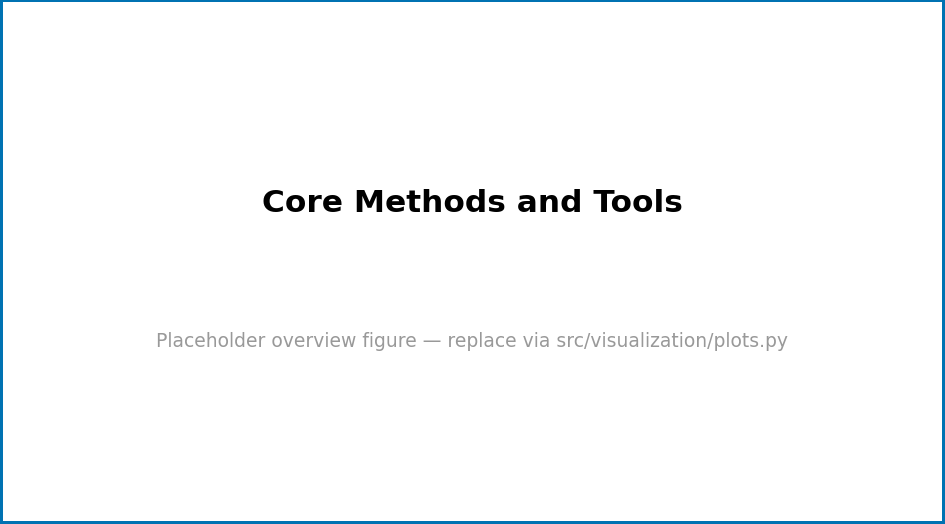
\includegraphics[width=0.9\linewidth,height=0.50\textheight,keepaspectratio,alt={Overview schematic for ``Core Methods and Tools''. Replace this generated placeholder with a real figure produced by src/visualization/plots.py.}]{../figures/part_0_core_methods.png}
\caption{Overview schematic for ``Core Methods and Tools''. Replace this
generated placeholder with a real figure produced by
\protect\breaktt{src/visualization/plots.py}.}\label{fig:part_0_core_methods}
\end{figure}

\begin{quote}
Level 1/3 \texorpdfstring{\ensuremath{\cdot}}{.} 30 min read \texorpdfstring{\ensuremath{\cdot}}{.} 45 min lecture \texorpdfstring{\ensuremath{\cdot}}{.} Prerequisites: none
\end{quote}

\subsection{Learning Objectives}\label{learning-objectives-1}

By the end of this chapter you should be able to:

\begin{enumerate}
\def\labelenumi{\arabic{enumi}.}
\item
  TODO: state the first measurable learning objective.
\item
  TODO: state the second learning objective.
\item
  TODO: state the third learning objective.
\end{enumerate}

\subsubsection{Study Blueprint}\label{study-blueprint-1}

\begin{itemize}
\tightlist
\item
  \textbf{Big idea:}
\item
  \textbf{Core concepts:} \hyperref[gl:model]{\textbf{model}},
  \hyperref[gl:parameter]{\textbf{parameter}},
  \hyperref[gl:variable]{\textbf{variable}}.
\item
  \textbf{Quantitative lens:} the worked formalism in
  eq.~\ref{eq:part_0_core_methods_model}.
\item
  \textbf{Data skill:}
\item
  \textbf{Common misconception to repair:}
\item
  \textbf{Primary lab:} sec.~\ref{sec:lab_part_0_core_methods}.
\item
  \textbf{Question bank:} sec.~\ref{sec:q_part_0_core_methods}.
\item
  \textbf{Bridge to computation:} \texttt{textbook.models}.
\end{itemize}

\begin{center}\rule{0.5\linewidth}{0.5pt}\end{center}

\begin{quote}
\textbf{Opening Vignette: TKTK --- a motivating story}
\end{quote}

\begin{center}\rule{0.5\linewidth}{0.5pt}\end{center}

\subsection{Orientation}\label{orientation-1}

This section introduces the central ideas of \emph{Core Methods and
Tools}. Foundational treatments include
\citep{kim2020data, brown2017principles}. Key terms such as
\hyperref[gl:model]{\textbf{model}},
\hyperref[gl:parameter]{\textbf{parameter}},
\hyperref[gl:variable]{\textbf{variable}} are defined in the glossary.

\subsection{A Worked Formalism}\label{a-worked-formalism-1}

The recurring quantitative model for this chapter is shown in
eq.~\ref{eq:part_0_core_methods_model}:

\begin{equation}\protect\phantomsection\label{eq:part_0_core_methods_model}{ N(t) = \frac{K}{1 + \left(\dfrac{K - N_0}{N_0}\right) e^{-rt}} }\end{equation}

It is implemented and tested in
\breaktt{textbook.models.logistic\_growth}; never retype the maths in
prose or scripts --- call the tested function. The parameters appear in
tbl.~\ref{tbl:part_0_core_methods_parameters}.

\begin{longtable}[]{@{}lll@{}}
\caption{Parameters of the worked model for this
chapter.}\label{tbl:part_0_core_methods_parameters}\tabularnewline
\toprule\noalign{}
Symbol & Meaning & Units \\
\midrule\noalign{}
\endfirsthead
\toprule\noalign{}
Symbol & Meaning & Units \\
\midrule\noalign{}
\endhead
\bottomrule\noalign{}
\endlastfoot
\(r\) & intrinsic rate & 1/time \\
\(K\) & carrying capacity & quantity \\
\(N_0\) & initial value & quantity \\
\end{longtable}

A concept map of how the pieces fit together:

\begin{figure}[htbp]
\centering
\begin{verbatim}
graph TD
  A[Inputs / assumptions] --> B[Model]
  B --> C[Predictions]
  C --> D[Comparison with data]
  D -->|revise| A
\end{verbatim}
\caption{Mermaid diagram}
\end{figure}

\begin{quote}
\textbf{Note}
\end{quote}

\subsection{Going Deeper}\label{going-deeper-1}

See the overview in fig.~\ref{fig:part_0_core_methods} and revisit the
objectives above as you read. Further evidence:
\citep{kim2020data, brown2017principles}.

\subsection{Summary}\label{summary-1}

\subsection{Key Terms}\label{key-terms-1}

\hyperref[gl:emergence]{\textbf{emergence}},
\hyperref[gl:regulation]{\textbf{regulation}},
\hyperref[gl:boundary]{\textbf{boundary}},
\hyperref[gl:state]{\textbf{state}}.

\subsection{Further Reading}\label{further-reading-1}

\begin{itemize}
\item
  TODO: one-line annotation \citep{wilson2021analysis}.
\end{itemize}

\subsection{Practice}\label{practice-1}

\begin{itemize}
\tightlist
\item
  \textbf{Lab:} sec.~\ref{sec:lab_part_0_core_methods}
\item
  \textbf{Question bank:} sec.~\ref{sec:q_part_0_core_methods}
\end{itemize}

\newpage

\section{Quantitative
Foundations}\label{sec:part_0_quantitative_foundations}

\begin{figure}
\centering

\includegraphics[width=0.9\linewidth,height=0.50\textheight,keepaspectratio,alt={Overview schematic for ``Quantitative Foundations''. Replace this generated placeholder with a real figure produced by src/visualization/plots.py.}]{../figures/part_0_quantitative_foundations.png}
\caption{Overview schematic for ``Quantitative Foundations''. Replace
this generated placeholder with a real figure produced by
\protect\breaktt{src/visualization/plots.py}.}\label{fig:part_0_quantitative_foundations}
\end{figure}

\begin{quote}
Level 1/3 \texorpdfstring{\ensuremath{\cdot}}{.} 30 min read \texorpdfstring{\ensuremath{\cdot}}{.} 45 min lecture \texorpdfstring{\ensuremath{\cdot}}{.} Prerequisites: none
\end{quote}

\subsection{Learning Objectives}\label{learning-objectives-2}

By the end of this chapter you should be able to:

\begin{enumerate}
\def\labelenumi{\arabic{enumi}.}
\item
  TODO: state the first measurable learning objective.
\item
  TODO: state the second learning objective.
\item
  TODO: state the third learning objective.
\end{enumerate}

\subsubsection{Study Blueprint}\label{study-blueprint-2}

\begin{itemize}
\tightlist
\item
  \textbf{Big idea:}
\item
  \textbf{Core concepts:} \hyperref[gl:feedback]{\textbf{feedback}},
  \hyperref[gl:gradient]{\textbf{gradient}},
  \hyperref[gl:threshold]{\textbf{threshold}}.
\item
  \textbf{Quantitative lens:} the worked formalism in
  eq.~\ref{eq:part_0_quantitative_foundations_model}.
\item
  \textbf{Data skill:}
\item
  \textbf{Common misconception to repair:}
\item
  \textbf{Primary lab:}
  sec.~\ref{sec:lab_part_0_quantitative_foundations}.
\item
  \textbf{Question bank:}
  sec.~\ref{sec:q_part_0_quantitative_foundations}.
\item
  \textbf{Bridge to computation:} \texttt{textbook.models}.
\end{itemize}

\begin{center}\rule{0.5\linewidth}{0.5pt}\end{center}

\begin{quote}
\textbf{Opening Vignette: TKTK --- a motivating story}
\end{quote}

\begin{center}\rule{0.5\linewidth}{0.5pt}\end{center}

\subsection{Orientation}\label{orientation-2}

This section introduces the central ideas of \emph{Quantitative
Foundations}. Foundational treatments include
\citep{smith2020foundations, doe2019methods}. Key terms such as
\hyperref[gl:feedback]{\textbf{feedback}},
\hyperref[gl:gradient]{\textbf{gradient}},
\hyperref[gl:threshold]{\textbf{threshold}} are defined in the glossary.

\subsection{A Worked Formalism}\label{a-worked-formalism-2}

The recurring quantitative model for this chapter is shown in
eq.~\ref{eq:part_0_quantitative_foundations_model}:

\begin{equation}\protect\phantomsection\label{eq:part_0_quantitative_foundations_model}{ N(t) = \frac{K}{1 + \left(\dfrac{K - N_0}{N_0}\right) e^{-rt}} }\end{equation}

It is implemented and tested in
\breaktt{textbook.models.logistic\_growth}; never retype the maths in
prose or scripts --- call the tested function. The parameters appear in
tbl.~\ref{tbl:part_0_quantitative_foundations_parameters}.

\begin{longtable}[]{@{}lll@{}}
\caption{Parameters of the worked model for this
chapter.}\label{tbl:part_0_quantitative_foundations_parameters}\tabularnewline
\toprule\noalign{}
Symbol & Meaning & Units \\
\midrule\noalign{}
\endfirsthead
\toprule\noalign{}
Symbol & Meaning & Units \\
\midrule\noalign{}
\endhead
\bottomrule\noalign{}
\endlastfoot
\(r\) & intrinsic rate & 1/time \\
\(K\) & carrying capacity & quantity \\
\(N_0\) & initial value & quantity \\
\end{longtable}

A concept map of how the pieces fit together:

\begin{figure}[htbp]
\centering
\begin{verbatim}
graph TD
  A[Inputs / assumptions] --> B[Model]
  B --> C[Predictions]
  C --> D[Comparison with data]
  D -->|revise| A
\end{verbatim}
\caption{Mermaid diagram}
\end{figure}

\begin{quote}
\textbf{Note}
\end{quote}

\subsection{Going Deeper}\label{going-deeper-2}

See the overview in fig.~\ref{fig:part_0_quantitative_foundations} and
revisit the objectives above as you read. Further evidence:
\citep{smith2020foundations, doe2019methods}.

\subsection{Summary}\label{summary-2}

\subsection{Key Terms}\label{key-terms-2}

\hyperref[gl:observable]{\textbf{observable}},
\hyperref[gl:system]{\textbf{system}},
\hyperref[gl:model]{\textbf{model}},
\hyperref[gl:parameter]{\textbf{parameter}}.

\subsection{Further Reading}\label{further-reading-2}

\begin{itemize}
\item
  TODO: one-line annotation \citep{lee2021systems}.
\end{itemize}

\subsection{Practice}\label{practice-2}

\begin{itemize}
\tightlist
\item
  \textbf{Lab:} sec.~\ref{sec:lab_part_0_quantitative_foundations}
\item
  \textbf{Question bank:}
  sec.~\ref{sec:q_part_0_quantitative_foundations}
\end{itemize}

\newpage

\section{Part I: Fundamentals}\label{sec:part_I_intro}

This part covers \textbf{fundamentals}. It contains the following
chapters:

\begin{itemize}
\tightlist
\item
  \emph{First Principles} --- sec.~\ref{sec:part_I_first_principles}
\item
  \emph{Building Blocks} --- sec.~\ref{sec:part_I_building_blocks}
\item
  \emph{Structure and Form} --- sec.~\ref{sec:part_I_structure_and_form}
\end{itemize}

\begin{quote}
\textbf{How to use this part.}
\end{quote}

\newpage

\section{First Principles}\label{sec:part_I_first_principles}

\begin{figure}
\centering
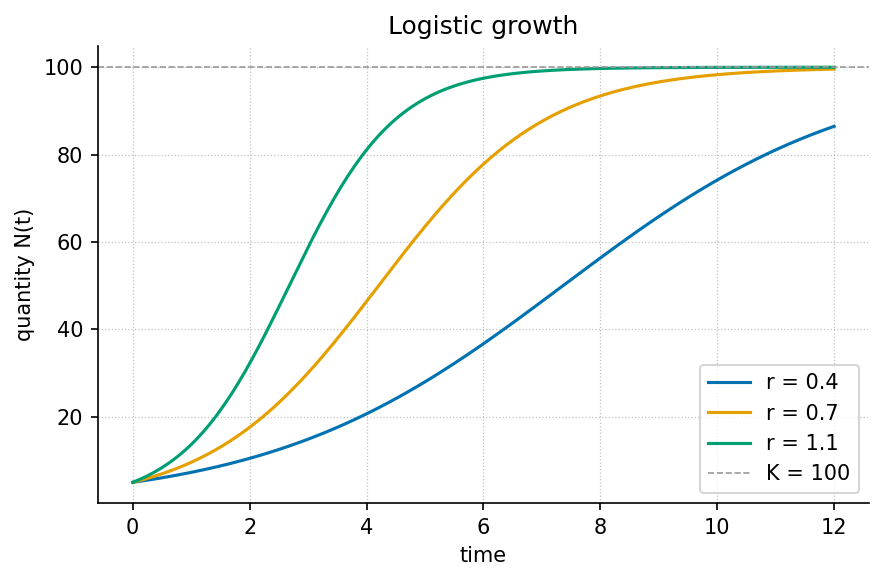
\includegraphics[width=0.85\linewidth,height=0.50\textheight,keepaspectratio,alt={A logistic growth curve for three growth rates, approaching the carrying capacity K = 100. Produced deterministically by visualization.plots.plot\_logistic\_growth.}]{../figures/logistic_growth.png}
\caption{A logistic growth curve for three growth rates, approaching the
carrying capacity \(K = 100\). Produced deterministically by
\protect\breaktt{visualization.plots.plot\_logistic\_growth}.}\label{fig:part_I_first_principles}
\end{figure}

\begin{quote}
Level 1/3 \texorpdfstring{\ensuremath{\cdot}}{.} 25 min read \texorpdfstring{\ensuremath{\cdot}}{.} 40 min lecture \texorpdfstring{\ensuremath{\cdot}}{.} Prerequisites: none
\end{quote}

\begin{quote}
\textbf{This chapter is a worked reference.} It is filled to completion
to show what a finished chapter looks like. The other chapters in this
template ship as structurally-complete stubs (marked with stub comments
and TODO notes); fill them the same way.
\end{quote}

\subsection{Learning Objectives}\label{learning-objectives-3}

By the end of this chapter you should be able to:

\begin{enumerate}
\def\labelenumi{\arabic{enumi}.}
\tightlist
\item
  Explain what it means to model a \hyperref[gl:system]{\textbf{system}}
  as a small set of \hyperref[gl:state]{\textbf{state}} variables and a
  rule for how they change.
\item
  Distinguish a \hyperref[gl:parameter]{\textbf{parameter}} from a
  \hyperref[gl:variable]{\textbf{variable}}, and identify each in a
  worked model.
\item
  Derive and interpret the logistic growth law and predict its long-run
  behaviour toward an \hyperref[gl:equilibrium]{\textbf{equilibrium}}.
\item
  Compute model values with the tested function
  \breaktt{textbook.models.logistic\_growth} rather than re-deriving
  arithmetic by hand.
\end{enumerate}

\subsubsection{Study Blueprint}\label{study-blueprint-3}

\begin{itemize}
\tightlist
\item
  \textbf{Big idea:} A great deal of change in the world is captured by
  a handful of variables and a single rule relating their rates --- the
  \emph{first principle} of quantitative modelling.
\item
  \textbf{Core concepts:} \hyperref[gl:system]{\textbf{system}},
  \hyperref[gl:state]{\textbf{state}},
  \hyperref[gl:parameter]{\textbf{parameter}},
  \hyperref[gl:equilibrium]{\textbf{equilibrium}}.
\item
  \textbf{Quantitative lens:} the logistic law in
  eq.~\ref{eq:part_I_first_principles_model}.
\item
  \textbf{Data skill:} read an S-curve and estimate its carrying
  capacity by eye, then confirm numerically.
\item
  \textbf{Common misconception to repair:} ``exponential'' and
  ``logistic'' are not the same --- unbounded growth is an early-time
  approximation, not the rule.
\item
  \textbf{Primary lab:} sec.~\ref{sec:lab_part_I_first_principles}.
\item
  \textbf{Question bank:} sec.~\ref{sec:q_part_I_first_principles}.
\item
  \textbf{Bridge to computation:}
  \breaktt{textbook.models.logistic\_growth}.
\end{itemize}

\begin{center}\rule{0.5\linewidth}{0.5pt}\end{center}

\begin{quote}
\textbf{Opening Vignette: Counting before you explain.}

A population biologist watches a colony double, then double again, then
--- unexpectedly --- slow. A start-up tracks users that grow the same
way before the market saturates. A chemist measures a reaction that
races, then crawls as substrate runs low. Three unrelated fields, one
shape. The job of a first model is not to capture everything; it is to
capture \emph{that shape} with as few moving parts as possible.
\end{quote}

\begin{center}\rule{0.5\linewidth}{0.5pt}\end{center}

\subsection{From a system to a model}\label{from-a-system-to-a-model}

A \textbf{model} is a deliberate simplification. We choose a small
number of \hyperref[gl:state]{\textbf{state}} variables --- here, a
single quantity \(N(t)\) --- and write a rule for how the state changes.
The art is leaving things out: a first model that fits on one line
teaches more than a faithful one that fills a page.

The variables are what change; the
\hyperref[gl:parameter]{\textbf{parameter}}s are what we hold fixed
while we reason. In the growth model below, \(N\) is the variable, while
the rate \(r\) and the carrying capacity \(K\) are parameters. Confusing
the two is the most common beginner error: if you find yourself
``solving for \(K\) over time,'' you have mislabelled a parameter as a
variable.

\subsection{A first quantitative law}\label{a-first-quantitative-law}

Unbounded (exponential) growth assumes nothing ever pushes back. Real
systems saturate. The simplest law that grows fast when small and levels
off when large is the \textbf{logistic} equation, written as a rate of
change in eq.~\ref{eq:part_I_first_principles_rate} and in closed form
in eq.~\ref{eq:part_I_first_principles_model}:

\begin{equation}\protect\phantomsection\label{eq:part_I_first_principles_rate}{ \frac{dN}{dt} = rN\left(1 - \frac{N}{K}\right) }\end{equation}

\begin{equation}\protect\phantomsection\label{eq:part_I_first_principles_model}{ N(t) = \frac{K}{1 + \left(\dfrac{K - N_0}{N_0}\right) e^{-rt}} }\end{equation}

Read eq.~\ref{eq:part_I_first_principles_rate} aloud: the rate of change
is proportional to how much there is (\(rN\)) \emph{times} how much room
remains (\(1 - N/K\)). When \(N\) is small the second factor is near
\(1\) and growth is nearly exponential; as \(N\) approaches \(K\) the
factor approaches \(0\) and growth stalls. The parameters are collected
in tbl.~\ref{tbl:part_I_first_principles_parameters}.

\begin{longtable}[]{@{}llll@{}}
\caption{Parameters of the logistic model. Variables change over time;
parameters are held fixed while
reasoning.}\label{tbl:part_I_first_principles_parameters}\tabularnewline
\toprule\noalign{}
Symbol & Name & Role & Example value \\
\midrule\noalign{}
\endfirsthead
\toprule\noalign{}
Symbol & Name & Role & Example value \\
\midrule\noalign{}
\endhead
\bottomrule\noalign{}
\endlastfoot
\(N(t)\) & quantity & variable & computed \\
\(r\) & intrinsic rate & parameter & \(0.8\ \mathrm{s^{-1}}\) \\
\(K\) & carrying capacity & parameter & \(100\) units \\
\(N_0\) & initial value & parameter & \(5\) units \\
\end{longtable}

\subsection{Worked example}\label{worked-example}

Take \(r = 0.8\), \(K = 100\), and \(N_0 = 5\). Rather than evaluate the
exponential by hand, call the tested backbone:

\begin{Shaded}
\begin{Highlighting}[]
\ImportTok{import}\NormalTok{ numpy }\ImportTok{as}\NormalTok{ np}
\ImportTok{from}\NormalTok{ textbook }\ImportTok{import}\NormalTok{ models}

\NormalTok{t }\OperatorTok{=}\NormalTok{ np.array([}\FloatTok{0.0}\NormalTok{, }\FloatTok{2.0}\NormalTok{, }\FloatTok{5.0}\NormalTok{, }\FloatTok{10.0}\NormalTok{])}
\NormalTok{N }\OperatorTok{=}\NormalTok{ models.logistic\_growth(t, r}\OperatorTok{=}\FloatTok{0.8}\NormalTok{, carrying\_capacity}\OperatorTok{=}\FloatTok{100.0}\NormalTok{, initial}\OperatorTok{=}\FloatTok{5.0}\NormalTok{)}
\CommentTok{\# N {-}\textgreater{} [ 5.00, 20.68, 74.18, 99.37 ]}
\end{Highlighting}
\end{Shaded}

The trajectory starts at \(N(0) = 5.00\), reaches \(N(2) = 20.68\),
passes the steep middle near \(t = 5\) with \(N(5) = 74.18\), and by
\(t = 10\) has all but arrived at \(N(10) = 99.37\) --- within one part
in a hundred of the carrying capacity. This is the S-curve plotted in
fig.~\ref{fig:part_I_first_principles}: an early near-exponential rise,
an inflection, and a long approach to the asymptote.

The long-run behaviour is exact, not approximate. Because \(r > 0\), the
term \(e^{-rt} \to 0\), so \(N(t) \to K\). The proof is one line and is
recorded as Theorem 1 in sec.~\ref{sec:appendix_formalisms}; the same
fact is asserted numerically by the test suite, so the prose and the
code cannot silently disagree.

\subsection{How the pieces connect}\label{how-the-pieces-connect}

\begin{figure}[htbp]
\centering
\begin{verbatim}
graph TD
  A[Choose state variables] --> B[Write a rate rule]
  B --> C[Solve or simulate]
  C --> D[Predict long-run behaviour]
  D -->|compare to data| A
\end{verbatim}
\caption{Mermaid diagram}
\end{figure}

This loop --- choose, write, solve, predict, compare --- is the first
principle the rest of the book elaborates. Foundational treatments of
model-building include \citep{brown2017principles} and
\citep{patel2018models}.

\subsection{Summary}\label{summary-3}

A model trades completeness for clarity: a few
\hyperref[gl:state]{\textbf{state}} variables and one rule. The logistic
law adds a single idea --- finite room --- to exponential growth, and
that idea changes the long-run behaviour from unbounded increase to a
stable \hyperref[gl:equilibrium]{\textbf{equilibrium}} at the carrying
capacity \(K\). Compute with the tested \texttt{logistic\_growth}
function so your worked numbers are reproducible and correct by
construction.

\subsection{Key Terms}\label{key-terms-3}

\hyperref[gl:system]{\textbf{system}},
\hyperref[gl:model]{\textbf{model}},
\hyperref[gl:state]{\textbf{state}},
\hyperref[gl:parameter]{\textbf{parameter}},
\hyperref[gl:equilibrium]{\textbf{equilibrium}}.

\subsection{Further Reading}\label{further-reading-3}

\begin{itemize}
\tightlist
\item
  \citet{brown2017principles} --- a readable introduction to reasoning
  from first principles; start with its opening chapter on what a model
  is for.
\item
  \citet{patel2018models} --- a broader survey of model families; use it
  to see where the logistic law sits among alternatives.
\end{itemize}

\subsection{Practice}\label{practice-3}

\begin{itemize}
\tightlist
\item
  \textbf{Lab:} sec.~\ref{sec:lab_part_I_first_principles} --- measure
  an S-curve and estimate its parameters.
\item
  \textbf{Question bank:} sec.~\ref{sec:q_part_I_first_principles} ---
  recall through synthesis.
\end{itemize}

\newpage

\section{Building Blocks}\label{sec:part_I_building_blocks}

\begin{figure}
\centering
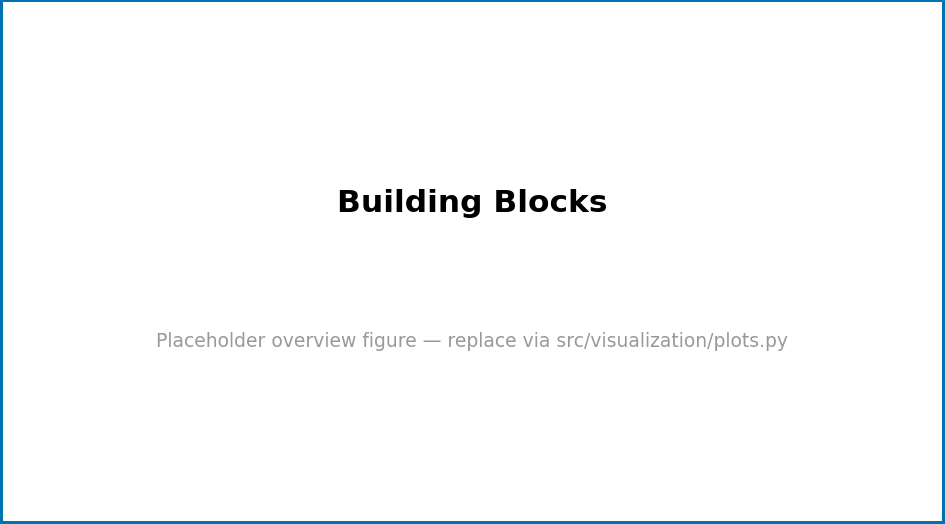
\includegraphics[width=0.9\linewidth,height=0.50\textheight,keepaspectratio,alt={Overview schematic for ``Building Blocks''. Replace this generated placeholder with a real figure produced by src/visualization/plots.py.}]{../figures/part_I_building_blocks.png}
\caption{Overview schematic for ``Building Blocks''. Replace this
generated placeholder with a real figure produced by
\protect\breaktt{src/visualization/plots.py}.}\label{fig:part_I_building_blocks}
\end{figure}

\begin{quote}
Level 1/3 \texorpdfstring{\ensuremath{\cdot}}{.} 30 min read \texorpdfstring{\ensuremath{\cdot}}{.} 45 min lecture \texorpdfstring{\ensuremath{\cdot}}{.} Prerequisites: none
\end{quote}

\subsection{Learning Objectives}\label{learning-objectives-4}

By the end of this chapter you should be able to:

\begin{enumerate}
\def\labelenumi{\arabic{enumi}.}
\item
  TODO: state the first measurable learning objective.
\item
  TODO: state the second learning objective.
\item
  TODO: state the third learning objective.
\end{enumerate}

\subsubsection{Study Blueprint}\label{study-blueprint-4}

\begin{itemize}
\tightlist
\item
  \textbf{Big idea:}
\item
  \textbf{Core concepts:}
  \hyperref[gl:equilibrium]{\textbf{equilibrium}},
  \hyperref[gl:feedback]{\textbf{feedback}},
  \hyperref[gl:gradient]{\textbf{gradient}}.
\item
  \textbf{Quantitative lens:} the worked formalism in
  eq.~\ref{eq:part_I_building_blocks_model}.
\item
  \textbf{Data skill:}
\item
  \textbf{Common misconception to repair:}
\item
  \textbf{Primary lab:} sec.~\ref{sec:lab_part_I_building_blocks}.
\item
  \textbf{Question bank:} sec.~\ref{sec:q_part_I_building_blocks}.
\item
  \textbf{Bridge to computation:} \texttt{textbook.models}.
\end{itemize}

\begin{center}\rule{0.5\linewidth}{0.5pt}\end{center}

\begin{quote}
\textbf{Opening Vignette: TKTK --- a motivating story}
\end{quote}

\begin{center}\rule{0.5\linewidth}{0.5pt}\end{center}

\subsection{Orientation}\label{orientation-3}

This section introduces the central ideas of \emph{Building Blocks}.
Foundational treatments include
\citep{taylor2019theory, smith2020foundations}. Key terms such as
\hyperref[gl:equilibrium]{\textbf{equilibrium}},
\hyperref[gl:feedback]{\textbf{feedback}},
\hyperref[gl:gradient]{\textbf{gradient}} are defined in the glossary.

\subsection{A Worked Formalism}\label{a-worked-formalism-3}

The recurring quantitative model for this chapter is shown in
eq.~\ref{eq:part_I_building_blocks_model}:

\begin{equation}\protect\phantomsection\label{eq:part_I_building_blocks_model}{ N(t) = \frac{K}{1 + \left(\dfrac{K - N_0}{N_0}\right) e^{-rt}} }\end{equation}

It is implemented and tested in
\breaktt{textbook.models.logistic\_growth}; never retype the maths in
prose or scripts --- call the tested function. The parameters appear in
tbl.~\ref{tbl:part_I_building_blocks_parameters}.

\begin{longtable}[]{@{}lll@{}}
\caption{Parameters of the worked model for this
chapter.}\label{tbl:part_I_building_blocks_parameters}\tabularnewline
\toprule\noalign{}
Symbol & Meaning & Units \\
\midrule\noalign{}
\endfirsthead
\toprule\noalign{}
Symbol & Meaning & Units \\
\midrule\noalign{}
\endhead
\bottomrule\noalign{}
\endlastfoot
\(r\) & intrinsic rate & 1/time \\
\(K\) & carrying capacity & quantity \\
\(N_0\) & initial value & quantity \\
\end{longtable}

A concept map of how the pieces fit together:

\begin{figure}[htbp]
\centering
\begin{verbatim}
graph TD
  A[Inputs / assumptions] --> B[Model]
  B --> C[Predictions]
  C --> D[Comparison with data]
  D -->|revise| A
\end{verbatim}
\caption{Mermaid diagram}
\end{figure}

\begin{quote}
\textbf{Note}
\end{quote}

\subsection{Going Deeper}\label{going-deeper-3}

See the overview in fig.~\ref{fig:part_I_building_blocks} and revisit
the objectives above as you read. Further evidence:
\citep{taylor2019theory, smith2020foundations}.

\subsection{Summary}\label{summary-4}

\subsection{Key Terms}\label{key-terms-4}

\hyperref[gl:state]{\textbf{state}},
\hyperref[gl:observable]{\textbf{observable}},
\hyperref[gl:system]{\textbf{system}},
\hyperref[gl:model]{\textbf{model}}.

\subsection{Further Reading}\label{further-reading-4}

\begin{itemize}
\item
  TODO: one-line annotation \citep{doe2019methods}.
\end{itemize}

\subsection{Practice}\label{practice-4}

\begin{itemize}
\tightlist
\item
  \textbf{Lab:} sec.~\ref{sec:lab_part_I_building_blocks}
\item
  \textbf{Question bank:} sec.~\ref{sec:q_part_I_building_blocks}
\end{itemize}

\newpage

\section{Structure and Form}\label{sec:part_I_structure_and_form}

\begin{figure}
\centering

\includegraphics[width=0.9\linewidth,height=0.50\textheight,keepaspectratio,alt={Overview schematic for ``Structure and Form''. Replace this generated placeholder with a real figure produced by src/visualization/plots.py.}]{../figures/part_I_structure_and_form.png}
\caption{Overview schematic for ``Structure and Form''. Replace this
generated placeholder with a real figure produced by
\protect\breaktt{src/visualization/plots.py}.}\label{fig:part_I_structure_and_form}
\end{figure}

\begin{quote}
Level 1/3 \texorpdfstring{\ensuremath{\cdot}}{.} 30 min read \texorpdfstring{\ensuremath{\cdot}}{.} 45 min lecture \texorpdfstring{\ensuremath{\cdot}}{.} Prerequisites: none
\end{quote}

\subsection{Learning Objectives}\label{learning-objectives-5}

By the end of this chapter you should be able to:

\begin{enumerate}
\def\labelenumi{\arabic{enumi}.}
\item
  TODO: state the first measurable learning objective.
\item
  TODO: state the second learning objective.
\item
  TODO: state the third learning objective.
\end{enumerate}

\subsubsection{Study Blueprint}\label{study-blueprint-5}

\begin{itemize}
\tightlist
\item
  \textbf{Big idea:}
\item
  \textbf{Core concepts:} \hyperref[gl:threshold]{\textbf{threshold}},
  \hyperref[gl:network]{\textbf{network}},
  \hyperref[gl:dynamics]{\textbf{dynamics}}.
\item
  \textbf{Quantitative lens:} the worked formalism in
  eq.~\ref{eq:part_I_structure_and_form_model}.
\item
  \textbf{Data skill:}
\item
  \textbf{Common misconception to repair:}
\item
  \textbf{Primary lab:} sec.~\ref{sec:lab_part_I_structure_and_form}.
\item
  \textbf{Question bank:} sec.~\ref{sec:q_part_I_structure_and_form}.
\item
  \textbf{Bridge to computation:} \texttt{textbook.models}.
\end{itemize}

\begin{center}\rule{0.5\linewidth}{0.5pt}\end{center}

\begin{quote}
\textbf{Opening Vignette: TKTK --- a motivating story}
\end{quote}

\begin{center}\rule{0.5\linewidth}{0.5pt}\end{center}

\subsection{Orientation}\label{orientation-4}

This section introduces the central ideas of \emph{Structure and Form}.
Foundational treatments include
\citep{lee2021systems, garcia2022dynamics}. Key terms such as
\hyperref[gl:threshold]{\textbf{threshold}},
\hyperref[gl:network]{\textbf{network}},
\hyperref[gl:dynamics]{\textbf{dynamics}} are defined in the glossary.

\subsection{A Worked Formalism}\label{a-worked-formalism-4}

The recurring quantitative model for this chapter is shown in
eq.~\ref{eq:part_I_structure_and_form_model}:

\begin{equation}\protect\phantomsection\label{eq:part_I_structure_and_form_model}{ N(t) = \frac{K}{1 + \left(\dfrac{K - N_0}{N_0}\right) e^{-rt}} }\end{equation}

It is implemented and tested in
\breaktt{textbook.models.logistic\_growth}; never retype the maths in
prose or scripts --- call the tested function. The parameters appear in
tbl.~\ref{tbl:part_I_structure_and_form_parameters}.

\begin{longtable}[]{@{}lll@{}}
\caption{Parameters of the worked model for this
chapter.}\label{tbl:part_I_structure_and_form_parameters}\tabularnewline
\toprule\noalign{}
Symbol & Meaning & Units \\
\midrule\noalign{}
\endfirsthead
\toprule\noalign{}
Symbol & Meaning & Units \\
\midrule\noalign{}
\endhead
\bottomrule\noalign{}
\endlastfoot
\(r\) & intrinsic rate & 1/time \\
\(K\) & carrying capacity & quantity \\
\(N_0\) & initial value & quantity \\
\end{longtable}

A concept map of how the pieces fit together:

\begin{figure}[htbp]
\centering
\begin{verbatim}
graph TD
  A[Inputs / assumptions] --> B[Model]
  B --> C[Predictions]
  C --> D[Comparison with data]
  D -->|revise| A
\end{verbatim}
\caption{Mermaid diagram}
\end{figure}

\begin{quote}
\textbf{Note}
\end{quote}

\subsection{Going Deeper}\label{going-deeper-4}

See the overview in fig.~\ref{fig:part_I_structure_and_form} and revisit
the objectives above as you read. Further evidence:
\citep{lee2021systems, garcia2022dynamics}.

\subsection{Summary}\label{summary-5}

\subsection{Key Terms}\label{key-terms-5}

\hyperref[gl:model]{\textbf{model}},
\hyperref[gl:parameter]{\textbf{parameter}},
\hyperref[gl:variable]{\textbf{variable}},
\hyperref[gl:equilibrium]{\textbf{equilibrium}}.

\subsection{Further Reading}\label{further-reading-5}

\begin{itemize}
\item
  TODO: one-line annotation \citep{patel2018models}.
\end{itemize}

\subsection{Practice}\label{practice-5}

\begin{itemize}
\tightlist
\item
  \textbf{Lab:} sec.~\ref{sec:lab_part_I_structure_and_form}
\item
  \textbf{Question bank:} sec.~\ref{sec:q_part_I_structure_and_form}
\end{itemize}

\newpage

\section{Part II: Core Systems}\label{sec:part_II_intro}

This part covers \textbf{core systems}. It contains the following
chapters:

\begin{itemize}
\tightlist
\item
  \emph{Systems Overview} --- sec.~\ref{sec:part_II_systems_overview}
\item
  \emph{Dynamics and Change} ---
  sec.~\ref{sec:part_II_dynamics_and_change}
\item
  \emph{Regulation and Control} ---
  sec.~\ref{sec:part_II_regulation_and_control}
\end{itemize}

\begin{quote}
\textbf{How to use this part.}
\end{quote}

\newpage

\section{Systems Overview}\label{sec:part_II_systems_overview}

\begin{figure}
\centering
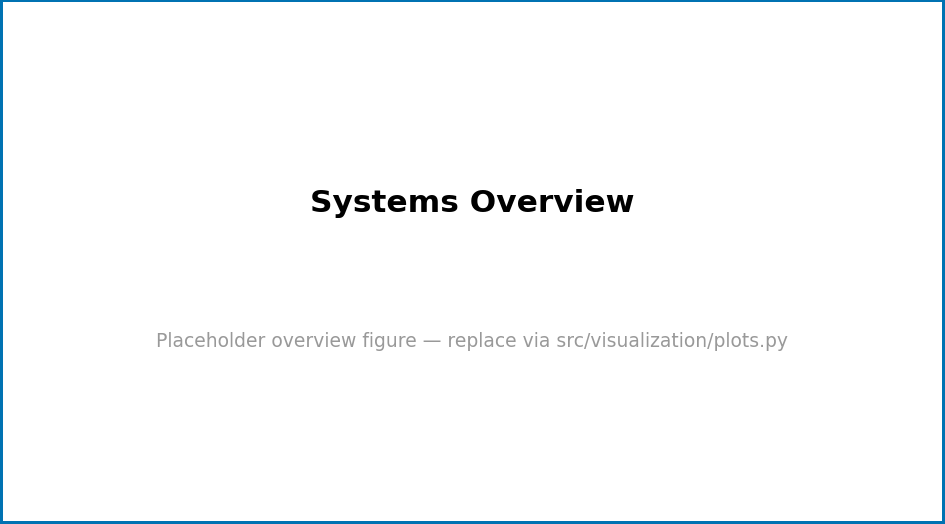
\includegraphics[width=0.9\linewidth,height=0.50\textheight,keepaspectratio,alt={Overview schematic for ``Systems Overview''. Replace this generated placeholder with a real figure produced by src/visualization/plots.py.}]{../figures/part_II_systems_overview.png}
\caption{Overview schematic for ``Systems Overview''. Replace this
generated placeholder with a real figure produced by
\protect\breaktt{src/visualization/plots.py}.}\label{fig:part_II_systems_overview}
\end{figure}

\begin{quote}
Level 1/3 \texorpdfstring{\ensuremath{\cdot}}{.} 30 min read \texorpdfstring{\ensuremath{\cdot}}{.} 45 min lecture \texorpdfstring{\ensuremath{\cdot}}{.} Prerequisites: none
\end{quote}

\subsection{Learning Objectives}\label{learning-objectives-6}

By the end of this chapter you should be able to:

\begin{enumerate}
\def\labelenumi{\arabic{enumi}.}
\item
  TODO: state the first measurable learning objective.
\item
  TODO: state the second learning objective.
\item
  TODO: state the third learning objective.
\end{enumerate}

\subsubsection{Study Blueprint}\label{study-blueprint-6}

\begin{itemize}
\tightlist
\item
  \textbf{Big idea:}
\item
  \textbf{Core concepts:}
  \hyperref[gl:equilibrium]{\textbf{equilibrium}},
  \hyperref[gl:feedback]{\textbf{feedback}},
  \hyperref[gl:gradient]{\textbf{gradient}}.
\item
  \textbf{Quantitative lens:} the worked formalism in
  eq.~\ref{eq:part_II_systems_overview_model}.
\item
  \textbf{Data skill:}
\item
  \textbf{Common misconception to repair:}
\item
  \textbf{Primary lab:} sec.~\ref{sec:lab_part_II_systems_overview}.
\item
  \textbf{Question bank:} sec.~\ref{sec:q_part_II_systems_overview}.
\item
  \textbf{Bridge to computation:} \texttt{textbook.models}.
\end{itemize}

\begin{center}\rule{0.5\linewidth}{0.5pt}\end{center}

\begin{quote}
\textbf{Opening Vignette: TKTK --- a motivating story}
\end{quote}

\begin{center}\rule{0.5\linewidth}{0.5pt}\end{center}

\subsection{Orientation}\label{orientation-5}

This section introduces the central ideas of \emph{Systems Overview}.
Foundational treatments include
\citep{patel2018models, nguyen2023synthesis}. Key terms such as
\hyperref[gl:equilibrium]{\textbf{equilibrium}},
\hyperref[gl:feedback]{\textbf{feedback}},
\hyperref[gl:gradient]{\textbf{gradient}} are defined in the glossary.

\subsection{A Worked Formalism}\label{a-worked-formalism-5}

The recurring quantitative model for this chapter is shown in
eq.~\ref{eq:part_II_systems_overview_model}:

\begin{equation}\protect\phantomsection\label{eq:part_II_systems_overview_model}{ N(t) = \frac{K}{1 + \left(\dfrac{K - N_0}{N_0}\right) e^{-rt}} }\end{equation}

It is implemented and tested in
\breaktt{textbook.models.logistic\_growth}; never retype the maths in
prose or scripts --- call the tested function. The parameters appear in
tbl.~\ref{tbl:part_II_systems_overview_parameters}.

\begin{longtable}[]{@{}lll@{}}
\caption{Parameters of the worked model for this
chapter.}\label{tbl:part_II_systems_overview_parameters}\tabularnewline
\toprule\noalign{}
Symbol & Meaning & Units \\
\midrule\noalign{}
\endfirsthead
\toprule\noalign{}
Symbol & Meaning & Units \\
\midrule\noalign{}
\endhead
\bottomrule\noalign{}
\endlastfoot
\(r\) & intrinsic rate & 1/time \\
\(K\) & carrying capacity & quantity \\
\(N_0\) & initial value & quantity \\
\end{longtable}

A concept map of how the pieces fit together:

\begin{figure}[htbp]
\centering
\begin{verbatim}
graph TD
  A[Inputs / assumptions] --> B[Model]
  B --> C[Predictions]
  C --> D[Comparison with data]
  D -->|revise| A
\end{verbatim}
\caption{Mermaid diagram}
\end{figure}

\begin{quote}
\textbf{Note}
\end{quote}

\subsection{Going Deeper}\label{going-deeper-5}

See the overview in fig.~\ref{fig:part_II_systems_overview} and revisit
the objectives above as you read. Further evidence:
\citep{patel2018models, nguyen2023synthesis}.

\subsection{Summary}\label{summary-6}

\subsection{Key Terms}\label{key-terms-6}

\hyperref[gl:state]{\textbf{state}},
\hyperref[gl:observable]{\textbf{observable}},
\hyperref[gl:system]{\textbf{system}},
\hyperref[gl:model]{\textbf{model}}.

\subsection{Further Reading}\label{further-reading-6}

\begin{itemize}
\item
  TODO: one-line annotation \citep{kim2020data}.
\end{itemize}

\subsection{Practice}\label{practice-6}

\begin{itemize}
\tightlist
\item
  \textbf{Lab:} sec.~\ref{sec:lab_part_II_systems_overview}
\item
  \textbf{Question bank:} sec.~\ref{sec:q_part_II_systems_overview}
\end{itemize}

\newpage

\section{Dynamics and Change}\label{sec:part_II_dynamics_and_change}

\begin{figure}
\centering
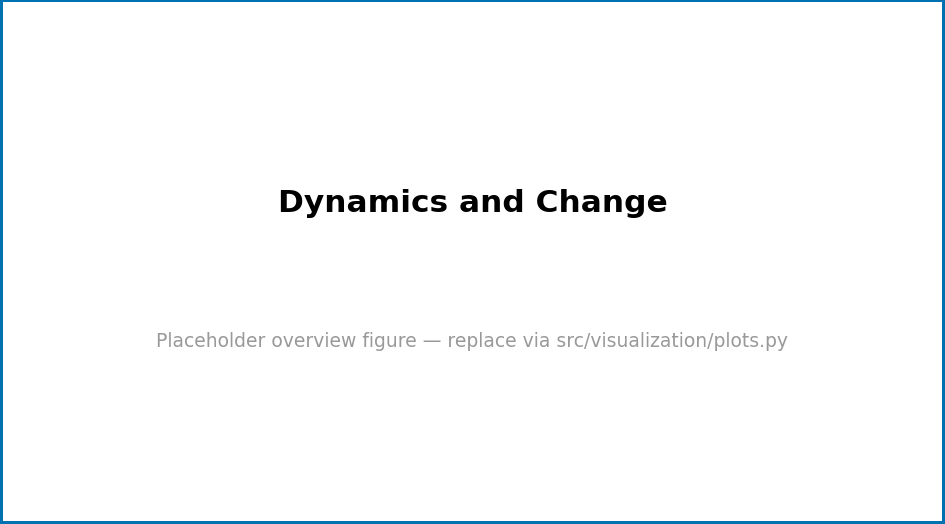
\includegraphics[width=0.9\linewidth,height=0.50\textheight,keepaspectratio,alt={Overview schematic for ``Dynamics and Change''. Replace this generated placeholder with a real figure produced by src/visualization/plots.py.}]{../figures/part_II_dynamics_and_change.png}
\caption{Overview schematic for ``Dynamics and Change''. Replace this
generated placeholder with a real figure produced by
\protect\breaktt{src/visualization/plots.py}.}\label{fig:part_II_dynamics_and_change}
\end{figure}

\begin{quote}
Level 1/3 \texorpdfstring{\ensuremath{\cdot}}{.} 30 min read \texorpdfstring{\ensuremath{\cdot}}{.} 45 min lecture \texorpdfstring{\ensuremath{\cdot}}{.} Prerequisites: none
\end{quote}

\subsection{Learning Objectives}\label{learning-objectives-7}

By the end of this chapter you should be able to:

\begin{enumerate}
\def\labelenumi{\arabic{enumi}.}
\item
  TODO: state the first measurable learning objective.
\item
  TODO: state the second learning objective.
\item
  TODO: state the third learning objective.
\end{enumerate}

\subsubsection{Study Blueprint}\label{study-blueprint-7}

\begin{itemize}
\tightlist
\item
  \textbf{Big idea:}
\item
  \textbf{Core concepts:} \hyperref[gl:parameter]{\textbf{parameter}},
  \hyperref[gl:variable]{\textbf{variable}},
  \hyperref[gl:equilibrium]{\textbf{equilibrium}}.
\item
  \textbf{Quantitative lens:} the worked formalism in
  eq.~\ref{eq:part_II_dynamics_and_change_model}.
\item
  \textbf{Data skill:}
\item
  \textbf{Common misconception to repair:}
\item
  \textbf{Primary lab:} sec.~\ref{sec:lab_part_II_dynamics_and_change}.
\item
  \textbf{Question bank:} sec.~\ref{sec:q_part_II_dynamics_and_change}.
\item
  \textbf{Bridge to computation:} \texttt{textbook.models}.
\end{itemize}

\begin{center}\rule{0.5\linewidth}{0.5pt}\end{center}

\begin{quote}
\textbf{Opening Vignette: TKTK --- a motivating story}
\end{quote}

\begin{center}\rule{0.5\linewidth}{0.5pt}\end{center}

\subsection{Orientation}\label{orientation-6}

This section introduces the central ideas of \emph{Dynamics and Change}.
Foundational treatments include
\citep{brown2017principles, wilson2021analysis}. Key terms such as
\hyperref[gl:parameter]{\textbf{parameter}},
\hyperref[gl:variable]{\textbf{variable}},
\hyperref[gl:equilibrium]{\textbf{equilibrium}} are defined in the
glossary.

\subsection{A Worked Formalism}\label{a-worked-formalism-6}

The recurring quantitative model for this chapter is shown in
eq.~\ref{eq:part_II_dynamics_and_change_model}:

\begin{equation}\protect\phantomsection\label{eq:part_II_dynamics_and_change_model}{ N(t) = \frac{K}{1 + \left(\dfrac{K - N_0}{N_0}\right) e^{-rt}} }\end{equation}

It is implemented and tested in
\breaktt{textbook.models.logistic\_growth}; never retype the maths in
prose or scripts --- call the tested function. The parameters appear in
tbl.~\ref{tbl:part_II_dynamics_and_change_parameters}.

\begin{longtable}[]{@{}lll@{}}
\caption{Parameters of the worked model for this
chapter.}\label{tbl:part_II_dynamics_and_change_parameters}\tabularnewline
\toprule\noalign{}
Symbol & Meaning & Units \\
\midrule\noalign{}
\endfirsthead
\toprule\noalign{}
Symbol & Meaning & Units \\
\midrule\noalign{}
\endhead
\bottomrule\noalign{}
\endlastfoot
\(r\) & intrinsic rate & 1/time \\
\(K\) & carrying capacity & quantity \\
\(N_0\) & initial value & quantity \\
\end{longtable}

A concept map of how the pieces fit together:

\begin{figure}[htbp]
\centering
\begin{verbatim}
graph TD
  A[Inputs / assumptions] --> B[Model]
  B --> C[Predictions]
  C --> D[Comparison with data]
  D -->|revise| A
\end{verbatim}
\caption{Mermaid diagram}
\end{figure}

\begin{quote}
\textbf{Note}
\end{quote}

\subsection{Going Deeper}\label{going-deeper-6}

See the overview in fig.~\ref{fig:part_II_dynamics_and_change} and
revisit the objectives above as you read. Further evidence:
\citep{brown2017principles, wilson2021analysis}.

\subsection{Summary}\label{summary-7}

\subsection{Key Terms}\label{key-terms-7}

\hyperref[gl:regulation]{\textbf{regulation}},
\hyperref[gl:boundary]{\textbf{boundary}},
\hyperref[gl:state]{\textbf{state}},
\hyperref[gl:observable]{\textbf{observable}}.

\subsection{Further Reading}\label{further-reading-7}

\begin{itemize}
\item
  TODO: one-line annotation \citep{taylor2019theory}.
\end{itemize}

\subsection{Practice}\label{practice-7}

\begin{itemize}
\tightlist
\item
  \textbf{Lab:} sec.~\ref{sec:lab_part_II_dynamics_and_change}
\item
  \textbf{Question bank:} sec.~\ref{sec:q_part_II_dynamics_and_change}
\end{itemize}

\newpage

\section{Regulation and
Control}\label{sec:part_II_regulation_and_control}

\begin{figure}
\centering
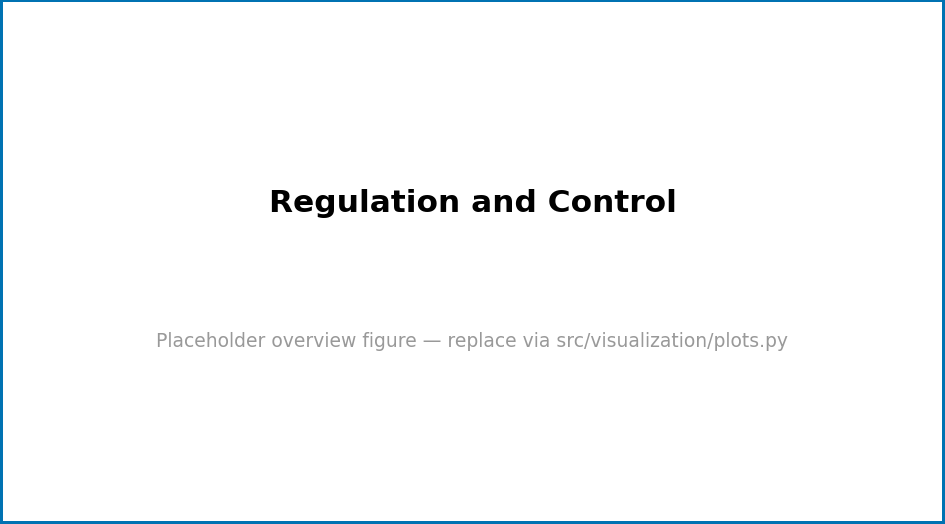
\includegraphics[width=0.9\linewidth,height=0.50\textheight,keepaspectratio,alt={Overview schematic for ``Regulation and Control''. Replace this generated placeholder with a real figure produced by src/visualization/plots.py.}]{../figures/part_II_regulation_and_control.png}
\caption{Overview schematic for ``Regulation and Control''. Replace this
generated placeholder with a real figure produced by
\protect\breaktt{src/visualization/plots.py}.}\label{fig:part_II_regulation_and_control}
\end{figure}

\begin{quote}
Level 1/3 \texorpdfstring{\ensuremath{\cdot}}{.} 30 min read \texorpdfstring{\ensuremath{\cdot}}{.} 45 min lecture \texorpdfstring{\ensuremath{\cdot}}{.} Prerequisites: none
\end{quote}

\subsection{Learning Objectives}\label{learning-objectives-8}

By the end of this chapter you should be able to:

\begin{enumerate}
\def\labelenumi{\arabic{enumi}.}
\item
  TODO: state the first measurable learning objective.
\item
  TODO: state the second learning objective.
\item
  TODO: state the third learning objective.
\end{enumerate}

\subsubsection{Study Blueprint}\label{study-blueprint-8}

\begin{itemize}
\tightlist
\item
  \textbf{Big idea:}
\item
  \textbf{Core concepts:} \hyperref[gl:network]{\textbf{network}},
  \hyperref[gl:dynamics]{\textbf{dynamics}},
  \hyperref[gl:emergence]{\textbf{emergence}}.
\item
  \textbf{Quantitative lens:} the worked formalism in
  eq.~\ref{eq:part_II_regulation_and_control_model}.
\item
  \textbf{Data skill:}
\item
  \textbf{Common misconception to repair:}
\item
  \textbf{Primary lab:}
  sec.~\ref{sec:lab_part_II_regulation_and_control}.
\item
  \textbf{Question bank:}
  sec.~\ref{sec:q_part_II_regulation_and_control}.
\item
  \textbf{Bridge to computation:} \texttt{textbook.models}.
\end{itemize}

\begin{center}\rule{0.5\linewidth}{0.5pt}\end{center}

\begin{quote}
\textbf{Opening Vignette: TKTK --- a motivating story}
\end{quote}

\begin{center}\rule{0.5\linewidth}{0.5pt}\end{center}

\subsection{Orientation}\label{orientation-7}

This section introduces the central ideas of \emph{Regulation and
Control}. Foundational treatments include
\citep{wilson2021analysis, taylor2019theory}. Key terms such as
\hyperref[gl:network]{\textbf{network}},
\hyperref[gl:dynamics]{\textbf{dynamics}},
\hyperref[gl:emergence]{\textbf{emergence}} are defined in the glossary.

\subsection{A Worked Formalism}\label{a-worked-formalism-7}

The recurring quantitative model for this chapter is shown in
eq.~\ref{eq:part_II_regulation_and_control_model}:

\begin{equation}\protect\phantomsection\label{eq:part_II_regulation_and_control_model}{ N(t) = \frac{K}{1 + \left(\dfrac{K - N_0}{N_0}\right) e^{-rt}} }\end{equation}

It is implemented and tested in
\breaktt{textbook.models.logistic\_growth}; never retype the maths in
prose or scripts --- call the tested function. The parameters appear in
tbl.~\ref{tbl:part_II_regulation_and_control_parameters}.

\begin{longtable}[]{@{}lll@{}}
\caption{Parameters of the worked model for this
chapter.}\label{tbl:part_II_regulation_and_control_parameters}\tabularnewline
\toprule\noalign{}
Symbol & Meaning & Units \\
\midrule\noalign{}
\endfirsthead
\toprule\noalign{}
Symbol & Meaning & Units \\
\midrule\noalign{}
\endhead
\bottomrule\noalign{}
\endlastfoot
\(r\) & intrinsic rate & 1/time \\
\(K\) & carrying capacity & quantity \\
\(N_0\) & initial value & quantity \\
\end{longtable}

A concept map of how the pieces fit together:

\begin{figure}[htbp]
\centering
\begin{verbatim}
graph TD
  A[Inputs / assumptions] --> B[Model]
  B --> C[Predictions]
  C --> D[Comparison with data]
  D -->|revise| A
\end{verbatim}
\caption{Mermaid diagram}
\end{figure}

\begin{quote}
\textbf{Note}
\end{quote}

\subsection{Going Deeper}\label{going-deeper-7}

See the overview in fig.~\ref{fig:part_II_regulation_and_control} and
revisit the objectives above as you read. Further evidence:
\citep{wilson2021analysis, taylor2019theory}.

\subsection{Summary}\label{summary-8}

\subsection{Key Terms}\label{key-terms-8}

\hyperref[gl:parameter]{\textbf{parameter}},
\hyperref[gl:variable]{\textbf{variable}},
\hyperref[gl:equilibrium]{\textbf{equilibrium}},
\hyperref[gl:feedback]{\textbf{feedback}}.

\subsection{Further Reading}\label{further-reading-8}

\begin{itemize}
\item
  TODO: one-line annotation \citep{smith2020foundations}.
\end{itemize}

\subsection{Practice}\label{practice-8}

\begin{itemize}
\tightlist
\item
  \textbf{Lab:} sec.~\ref{sec:lab_part_II_regulation_and_control}
\item
  \textbf{Question bank:}
  sec.~\ref{sec:q_part_II_regulation_and_control}
\end{itemize}

\newpage

\section{Part III: Applications and Synthesis}\label{sec:part_III_intro}

This part covers \textbf{applications and synthesis}. It contains the
following chapters:

\begin{itemize}
\tightlist
\item
  \emph{Applied Models} --- sec.~\ref{sec:part_III_applied_models}
\item
  \emph{Case Studies} --- sec.~\ref{sec:part_III_case_studies}
\item
  \emph{Frontiers and Open Problems} ---
  sec.~\ref{sec:part_III_frontiers}
\end{itemize}

\begin{quote}
\textbf{How to use this part.}
\end{quote}

\newpage

\section{Applied Models}\label{sec:part_III_applied_models}

\begin{figure}
\centering
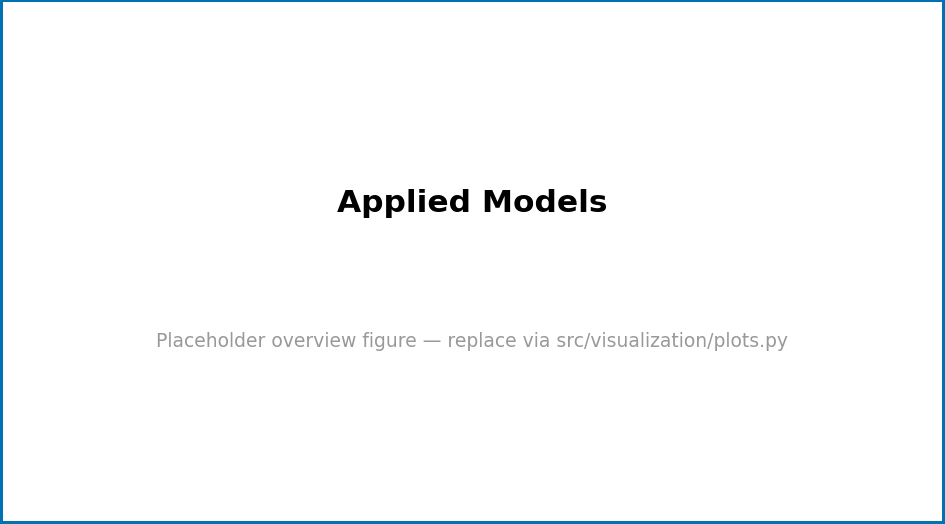
\includegraphics[width=0.9\linewidth,height=0.50\textheight,keepaspectratio,alt={Overview schematic for ``Applied Models''. Replace this generated placeholder with a real figure produced by src/visualization/plots.py.}]{../figures/part_III_applied_models.png}
\caption{Overview schematic for ``Applied Models''. Replace this
generated placeholder with a real figure produced by
\protect\breaktt{src/visualization/plots.py}.}\label{fig:part_III_applied_models}
\end{figure}

\begin{quote}
Level 1/3 \texorpdfstring{\ensuremath{\cdot}}{.} 30 min read \texorpdfstring{\ensuremath{\cdot}}{.} 45 min lecture \texorpdfstring{\ensuremath{\cdot}}{.} Prerequisites: none
\end{quote}

\subsection{Learning Objectives}\label{learning-objectives-9}

By the end of this chapter you should be able to:

\begin{enumerate}
\def\labelenumi{\arabic{enumi}.}
\item
  TODO: state the first measurable learning objective.
\item
  TODO: state the second learning objective.
\item
  TODO: state the third learning objective.
\end{enumerate}

\subsubsection{Study Blueprint}\label{study-blueprint-9}

\begin{itemize}
\tightlist
\item
  \textbf{Big idea:}
\item
  \textbf{Core concepts:}
  \hyperref[gl:equilibrium]{\textbf{equilibrium}},
  \hyperref[gl:feedback]{\textbf{feedback}},
  \hyperref[gl:gradient]{\textbf{gradient}}.
\item
  \textbf{Quantitative lens:} the worked formalism in
  eq.~\ref{eq:part_III_applied_models_model}.
\item
  \textbf{Data skill:}
\item
  \textbf{Common misconception to repair:}
\item
  \textbf{Primary lab:} sec.~\ref{sec:lab_part_III_applied_models}.
\item
  \textbf{Question bank:} sec.~\ref{sec:q_part_III_applied_models}.
\item
  \textbf{Bridge to computation:} \texttt{textbook.models}.
\end{itemize}

\begin{center}\rule{0.5\linewidth}{0.5pt}\end{center}

\begin{quote}
\textbf{Opening Vignette: TKTK --- a motivating story}
\end{quote}

\begin{center}\rule{0.5\linewidth}{0.5pt}\end{center}

\subsection{Orientation}\label{orientation-8}

This section introduces the central ideas of \emph{Applied Models}.
Foundational treatments include
\citep{patel2018models, nguyen2023synthesis}. Key terms such as
\hyperref[gl:equilibrium]{\textbf{equilibrium}},
\hyperref[gl:feedback]{\textbf{feedback}},
\hyperref[gl:gradient]{\textbf{gradient}} are defined in the glossary.

\subsection{A Worked Formalism}\label{a-worked-formalism-8}

The recurring quantitative model for this chapter is shown in
eq.~\ref{eq:part_III_applied_models_model}:

\begin{equation}\protect\phantomsection\label{eq:part_III_applied_models_model}{ N(t) = \frac{K}{1 + \left(\dfrac{K - N_0}{N_0}\right) e^{-rt}} }\end{equation}

It is implemented and tested in
\breaktt{textbook.models.logistic\_growth}; never retype the maths in
prose or scripts --- call the tested function. The parameters appear in
tbl.~\ref{tbl:part_III_applied_models_parameters}.

\begin{longtable}[]{@{}lll@{}}
\caption{Parameters of the worked model for this
chapter.}\label{tbl:part_III_applied_models_parameters}\tabularnewline
\toprule\noalign{}
Symbol & Meaning & Units \\
\midrule\noalign{}
\endfirsthead
\toprule\noalign{}
Symbol & Meaning & Units \\
\midrule\noalign{}
\endhead
\bottomrule\noalign{}
\endlastfoot
\(r\) & intrinsic rate & 1/time \\
\(K\) & carrying capacity & quantity \\
\(N_0\) & initial value & quantity \\
\end{longtable}

A concept map of how the pieces fit together:

\begin{figure}[htbp]
\centering
\begin{verbatim}
graph TD
  A[Inputs / assumptions] --> B[Model]
  B --> C[Predictions]
  C --> D[Comparison with data]
  D -->|revise| A
\end{verbatim}
\caption{Mermaid diagram}
\end{figure}

\begin{quote}
\textbf{Note}
\end{quote}

\subsection{Going Deeper}\label{going-deeper-8}

See the overview in fig.~\ref{fig:part_III_applied_models} and revisit
the objectives above as you read. Further evidence:
\citep{patel2018models, nguyen2023synthesis}.

\subsection{Summary}\label{summary-9}

\subsection{Key Terms}\label{key-terms-9}

\hyperref[gl:state]{\textbf{state}},
\hyperref[gl:observable]{\textbf{observable}},
\hyperref[gl:system]{\textbf{system}},
\hyperref[gl:model]{\textbf{model}}.

\subsection{Further Reading}\label{further-reading-9}

\begin{itemize}
\item
  TODO: one-line annotation \citep{kim2020data}.
\end{itemize}

\subsection{Practice}\label{practice-9}

\begin{itemize}
\tightlist
\item
  \textbf{Lab:} sec.~\ref{sec:lab_part_III_applied_models}
\item
  \textbf{Question bank:} sec.~\ref{sec:q_part_III_applied_models}
\end{itemize}

\newpage

\section{Case Studies}\label{sec:part_III_case_studies}

\begin{figure}
\centering
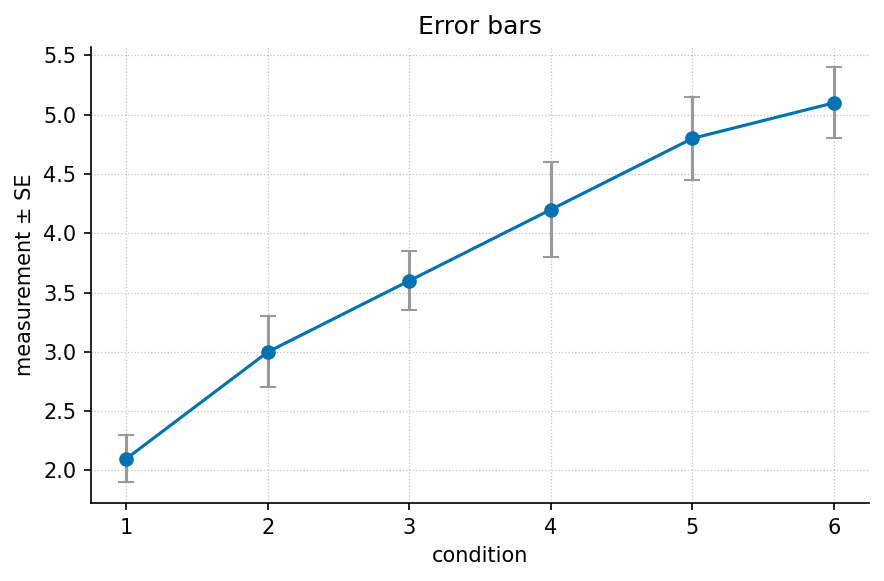
\includegraphics[width=0.75\linewidth,height=0.50\textheight,keepaspectratio,alt={Group means with standard-error bars across six synthetic conditions, generated by visualization.gallery.errorbar\_plot. In a real case study you would replace this gallery placeholder with your own measured group means.}]{../figures/gallery/gallery_errorbar.png}
\caption{Group means with standard-error bars across six synthetic
conditions, generated by
\protect\breaktt{visualization.gallery.errorbar\_plot}. In a real case
study you would replace this gallery placeholder with your own measured
group means.}\label{fig:part_III_case_studies}
\end{figure}

\begin{quote}
Level 2/3 \texorpdfstring{\ensuremath{\cdot}}{.} 30 min read \texorpdfstring{\ensuremath{\cdot}}{.} 45 min lecture \texorpdfstring{\ensuremath{\cdot}}{.} Prerequisites: First
Principles
\end{quote}

\begin{quote}
\textbf{This chapter is a worked reference} in a different style from
sec.~\ref{sec:part_I_first_principles}: where that chapter
\emph{derives} a model, this one \emph{applies} one to a small dataset.
The remaining chapters ship as stubs.
\end{quote}

\subsection{Learning Objectives}\label{learning-objectives-10}

By the end of this chapter you should be able to:

\begin{enumerate}
\def\labelenumi{\arabic{enumi}.}
\tightlist
\item
  Frame a real question as a comparison between a
  \hyperref[gl:system]{\textbf{system}} under control and treatment
  conditions.
\item
  Summarise grouped \hyperref[gl:observable]{\textbf{observable}} data
  with means and a measure of spread, and read an error-bar figure.
\item
  Fit a simple dose--response trend with
  \breaktt{textbook.models.linear\_fit} and state what its slope and
  \(R^2\) mean.
\item
  Distinguish a defensible interpolation from an unjustified
  extrapolation.
\end{enumerate}

\subsubsection{Study Blueprint}\label{study-blueprint-10}

\begin{itemize}
\tightlist
\item
  \textbf{Big idea:} A case study turns a general
  \hyperref[gl:model]{\textbf{model}} into a decision about a specific
  dataset --- and into an honest statement of its limits.
\item
  \textbf{Core concepts:} \hyperref[gl:observable]{\textbf{observable}},
  \hyperref[gl:gradient]{\textbf{gradient}},
  \hyperref[gl:threshold]{\textbf{threshold}}.
\item
  \textbf{Quantitative lens:} a linear dose--response fit,
  eq.~\ref{eq:part_III_case_studies_fit}.
\item
  \textbf{Data skill:} group, average, and fit; then sanity-check the
  fit against the raw numbers in
  tbl.~\ref{tbl:part_III_case_studies_data}.
\item
  \textbf{Common misconception to repair:} a high \(R^2\) on three
  points is not strong evidence --- it is an invitation to collect more.
\item
  \textbf{Primary lab:} sec.~\ref{sec:lab_part_III_case_studies}.
\item
  \textbf{Question bank:} sec.~\ref{sec:q_part_III_case_studies}.
\item
  \textbf{Bridge to computation:} \breaktt{textbook.models.linear\_fit},
  \breaktt{descriptive\_statistics}.
\end{itemize}

\begin{center}\rule{0.5\linewidth}{0.5pt}\end{center}

\begin{quote}
\textbf{Opening Vignette: From a spreadsheet to a decision.}

A team runs a small pilot: a control condition and two treatment levels,
two replicates each. The numbers land in a spreadsheet. The question is
not ``are they different?'' --- they obviously are --- but ``by how
much, how confidently, and what should we predict next?'' A case study
is the discipline of answering those three questions without
overreaching.
\end{quote}

\begin{center}\rule{0.5\linewidth}{0.5pt}\end{center}

\subsection{The data}\label{the-data}

The pilot produced six measurements across three conditions, recorded in
\breaktt{assets/data/sample\_dataset.csv} and reproduced in
tbl.~\ref{tbl:part_III_case_studies_data}.

\begin{longtable}[]{@{}lrrr@{}}
\caption{The pilot dataset: two replicates per
condition.}\label{tbl:part_III_case_studies_data}\tabularnewline
\toprule\noalign{}
Condition & Replicate & Measurement & Standard error \\
\midrule\noalign{}
\endfirsthead
\toprule\noalign{}
Condition & Replicate & Measurement & Standard error \\
\midrule\noalign{}
\endhead
\bottomrule\noalign{}
\endlastfoot
control & 1 & 2.10 & 0.20 \\
control & 2 & 2.30 & 0.18 \\
treatment (low) & 1 & 3.60 & 0.25 \\
treatment (low) & 2 & 3.40 & 0.22 \\
treatment (high) & 1 & 4.80 & 0.35 \\
treatment (high) & 2 & 5.10 & 0.30 \\
\end{longtable}

Grouping and averaging --- the first move in almost every case study ---
gives means of \(2.20\) (control), \(3.50\) (low), and \(4.95\) (high).
Across all six points the mean is \(3.55\) with a standard deviation of
\(1.13\) (\breaktt{textbook.models.descriptive\_statistics}). The
error-bar view is fig.~\ref{fig:part_III_case_studies}.

\subsection{Fitting a trend}\label{fitting-a-trend}

Encode the dose as \(0, 1, 2\) for control, low, and high, and fit a
line with \breaktt{textbook.models.linear\_fit}:

\begin{Shaded}
\begin{Highlighting}[]
\ImportTok{import}\NormalTok{ numpy }\ImportTok{as}\NormalTok{ np}
\ImportTok{from}\NormalTok{ textbook }\ImportTok{import}\NormalTok{ models}

\NormalTok{dose }\OperatorTok{=}\NormalTok{ np.array([}\FloatTok{0.0}\NormalTok{, }\FloatTok{1.0}\NormalTok{, }\FloatTok{2.0}\NormalTok{])}
\NormalTok{response }\OperatorTok{=}\NormalTok{ np.array([}\FloatTok{2.20}\NormalTok{, }\FloatTok{3.50}\NormalTok{, }\FloatTok{4.95}\NormalTok{])   }\CommentTok{\# condition means}
\NormalTok{fit }\OperatorTok{=}\NormalTok{ models.linear\_fit(dose, response)}
\CommentTok{\# fit.slope ≈ 1.375, fit.intercept ≈ 2.175, fit.r\_squared ≈ 0.999}
\end{Highlighting}
\end{Shaded}

The fitted relationship in eq.~\ref{eq:part_III_case_studies_fit} is

\begin{equation}\protect\phantomsection\label{eq:part_III_case_studies_fit}{ \widehat{y}(d) = 1.375\,d + 2.175 }\end{equation}

with \(R^2 = 0.999\). The slope says each dose step adds about \(1.4\)
units of response; the intercept, \(2.175\), is close to the measured
control mean of \(2.20\), a reassuring internal check.

\subsection{Interpolation versus
extrapolation}\label{interpolation-versus-extrapolation}

Using eq.~\ref{eq:part_III_case_studies_fit} to estimate the response at
an \emph{intermediate} dose is reasonable: the model interpolates within
the range it was fit on. Using it to predict a \emph{much higher} dose
--- say \(d = 3\), giving \(\widehat{y} = 6.3\) --- is an
\textbf{extrapolation} the data cannot support. Real dose--response
curves usually saturate (recall the
\hyperref[gl:threshold]{\textbf{threshold}} behaviour of the saturating
response in sec.~\ref{sec:part_I_first_principles}); a straight line
will overpredict once the system approaches its ceiling.

\begin{figure}[htbp]
\centering
\begin{verbatim}
graph LR
  A[Raw measurements] --> B[Group + average]
  B --> C[Fit a trend]
  C --> D{Within data range?}
  D -->|yes| E[Interpolate: defensible]
  D -->|no| F[Extrapolate: flag the risk]
\end{verbatim}
\caption{Mermaid diagram}
\end{figure}

\begin{quote}
\textbf{Warning.} A linear fit through three averaged points reports
\(R^2 = 0.999\), but that number describes how well the line passes
through three dots --- not how well it predicts the next experiment.
Treat it as a reason to collect more data, not as a conclusion.
Foundational guidance on this trap appears in \citep{kim2020data} and
\citep{wilson2021analysis}.
\end{quote}

\subsection{Summary}\label{summary-10}

A case study moves from raw
\hyperref[gl:observable]{\textbf{observable}}s to a summary, a fitted
trend, and --- crucially --- an honest boundary around what the trend
can claim. Here, averaging and a \texttt{linear\_fit} recovered a clean
dose--response slope of about \(1.4\) units per step with an intercept
that matched the control, but the same fit must not be pushed beyond the
measured range. The reusable move is: summarise, fit, then state the
limits.

\subsection{Key Terms}\label{key-terms-10}

\hyperref[gl:observable]{\textbf{observable}},
\hyperref[gl:gradient]{\textbf{gradient}},
\hyperref[gl:threshold]{\textbf{threshold}},
\hyperref[gl:model]{\textbf{model}}.

\subsection{Further Reading}\label{further-reading-10}

\begin{itemize}
\tightlist
\item
  \citet{kim2020data} --- practical guidance on summarising and
  visualising small datasets before fitting anything.
\item
  \citet{wilson2021analysis} --- on the difference between a good fit
  and a good prediction.
\end{itemize}

\subsection{Practice}\label{practice-10}

\begin{itemize}
\tightlist
\item
  \textbf{Lab:} sec.~\ref{sec:lab_part_III_case_studies} --- re-run the
  grouping and fit, then add a fourth condition and watch the fit
  change.
\item
  \textbf{Question bank:} sec.~\ref{sec:q_part_III_case_studies} ---
  recall through synthesis.
\end{itemize}

\newpage

\section{Frontiers and Open Problems}\label{sec:part_III_frontiers}

\begin{figure}
\centering

\includegraphics[width=0.9\linewidth,height=0.50\textheight,keepaspectratio,alt={Overview schematic for ``Frontiers and Open Problems''. Replace this generated placeholder with a real figure produced by src/visualization/plots.py.}]{../figures/part_III_frontiers.png}
\caption{Overview schematic for ``Frontiers and Open Problems''. Replace
this generated placeholder with a real figure produced by
\protect\breaktt{src/visualization/plots.py}.}\label{fig:part_III_frontiers}
\end{figure}

\begin{quote}
Level 1/3 \texorpdfstring{\ensuremath{\cdot}}{.} 30 min read \texorpdfstring{\ensuremath{\cdot}}{.} 45 min lecture \texorpdfstring{\ensuremath{\cdot}}{.} Prerequisites: none
\end{quote}

\subsection{Learning Objectives}\label{learning-objectives-11}

By the end of this chapter you should be able to:

\begin{enumerate}
\def\labelenumi{\arabic{enumi}.}
\item
  TODO: state the first measurable learning objective.
\item
  TODO: state the second learning objective.
\item
  TODO: state the third learning objective.
\end{enumerate}

\subsubsection{Study Blueprint}\label{study-blueprint-11}

\begin{itemize}
\tightlist
\item
  \textbf{Big idea:}
\item
  \textbf{Core concepts:} \hyperref[gl:state]{\textbf{state}},
  \hyperref[gl:observable]{\textbf{observable}},
  \hyperref[gl:system]{\textbf{system}}.
\item
  \textbf{Quantitative lens:} the worked formalism in
  eq.~\ref{eq:part_III_frontiers_model}.
\item
  \textbf{Data skill:}
\item
  \textbf{Common misconception to repair:}
\item
  \textbf{Primary lab:} sec.~\ref{sec:lab_part_III_frontiers}.
\item
  \textbf{Question bank:} sec.~\ref{sec:q_part_III_frontiers}.
\item
  \textbf{Bridge to computation:} \texttt{textbook.models}.
\end{itemize}

\begin{center}\rule{0.5\linewidth}{0.5pt}\end{center}

\begin{quote}
\textbf{Opening Vignette: TKTK --- a motivating story}
\end{quote}

\begin{center}\rule{0.5\linewidth}{0.5pt}\end{center}

\subsection{Orientation}\label{orientation-9}

This section introduces the central ideas of \emph{Frontiers and Open
Problems}. Foundational treatments include
\citep{wilson2021analysis, taylor2019theory}. Key terms such as
\hyperref[gl:state]{\textbf{state}},
\hyperref[gl:observable]{\textbf{observable}},
\hyperref[gl:system]{\textbf{system}} are defined in the glossary.

\subsection{A Worked Formalism}\label{a-worked-formalism-9}

The recurring quantitative model for this chapter is shown in
eq.~\ref{eq:part_III_frontiers_model}:

\begin{equation}\protect\phantomsection\label{eq:part_III_frontiers_model}{ N(t) = \frac{K}{1 + \left(\dfrac{K - N_0}{N_0}\right) e^{-rt}} }\end{equation}

It is implemented and tested in
\breaktt{textbook.models.logistic\_growth}; never retype the maths in
prose or scripts --- call the tested function. The parameters appear in
tbl.~\ref{tbl:part_III_frontiers_parameters}.

\begin{longtable}[]{@{}lll@{}}
\caption{Parameters of the worked model for this
chapter.}\label{tbl:part_III_frontiers_parameters}\tabularnewline
\toprule\noalign{}
Symbol & Meaning & Units \\
\midrule\noalign{}
\endfirsthead
\toprule\noalign{}
Symbol & Meaning & Units \\
\midrule\noalign{}
\endhead
\bottomrule\noalign{}
\endlastfoot
\(r\) & intrinsic rate & 1/time \\
\(K\) & carrying capacity & quantity \\
\(N_0\) & initial value & quantity \\
\end{longtable}

A concept map of how the pieces fit together:

\begin{figure}[htbp]
\centering
\begin{verbatim}
graph TD
  A[Inputs / assumptions] --> B[Model]
  B --> C[Predictions]
  C --> D[Comparison with data]
  D -->|revise| A
\end{verbatim}
\caption{Mermaid diagram}
\end{figure}

\begin{quote}
\textbf{Note}
\end{quote}

\subsection{Going Deeper}\label{going-deeper-9}

See the overview in fig.~\ref{fig:part_III_frontiers} and revisit the
objectives above as you read. Further evidence:
\citep{wilson2021analysis, taylor2019theory}.

\subsection{Summary}\label{summary-11}

\subsection{Key Terms}\label{key-terms-11}

\hyperref[gl:threshold]{\textbf{threshold}},
\hyperref[gl:network]{\textbf{network}},
\hyperref[gl:dynamics]{\textbf{dynamics}},
\hyperref[gl:emergence]{\textbf{emergence}}.

\subsection{Further Reading}\label{further-reading-11}

\begin{itemize}
\item
  TODO: one-line annotation \citep{smith2020foundations}.
\end{itemize}

\subsection{Practice}\label{practice-11}

\begin{itemize}
\tightlist
\item
  \textbf{Lab:} sec.~\ref{sec:lab_part_III_frontiers}
\item
  \textbf{Question bank:} sec.~\ref{sec:q_part_III_frontiers}
\end{itemize}

\newpage

\section{Lab --- Orientation to the
Field}\label{sec:lab_part_0_orientation}

\begin{quote}
Lab \texorpdfstring{\ensuremath{\cdot}}{.} 60 min \texorpdfstring{\ensuremath{\cdot}}{.} Materials: notebook, calculator (or
\texttt{textbook.models})
\end{quote}

\subsection{Objectives}\label{objectives}

\subsection{Background}\label{background}

Linked chapter: sec.~\ref{sec:part_0_orientation}.

\subsection{Procedure}\label{procedure}

\begin{enumerate}
\def\labelenumi{\arabic{enumi}.}
\item
  TODO: first step.
\item
  TODO: second step.
\end{enumerate}

\subsection{Analysis}\label{analysis}

Summarise results with \breaktt{textbook.models.descriptive\_statistics}.

\subsection{Computational Workflow}\label{computational-workflow}

\begin{Shaded}
\begin{Highlighting}[]
\ImportTok{from}\NormalTok{ textbook.models }\ImportTok{import}\NormalTok{ logistic\_growth}
\CommentTok{\# }\AlertTok{TODO}\CommentTok{: parameterise and plot the model for this lab\textquotesingle{}s scenario.}
\end{Highlighting}
\end{Shaded}

\subsection{Reflection}\label{reflection}

\newpage

\section{Lab --- Core Methods and
Tools}\label{sec:lab_part_0_core_methods}

\begin{quote}
Lab \texorpdfstring{\ensuremath{\cdot}}{.} 60 min \texorpdfstring{\ensuremath{\cdot}}{.} Materials: notebook, calculator (or
\texttt{textbook.models})
\end{quote}

\subsection{Objectives}\label{objectives-1}

\subsection{Background}\label{background-1}

Linked chapter: sec.~\ref{sec:part_0_core_methods}.

\subsection{Procedure}\label{procedure-1}

\begin{enumerate}
\def\labelenumi{\arabic{enumi}.}
\item
  TODO: first step.
\item
  TODO: second step.
\end{enumerate}

\subsection{Analysis}\label{analysis-1}

Summarise results with \breaktt{textbook.models.descriptive\_statistics}.

\subsection{Computational Workflow}\label{computational-workflow-1}

\begin{Shaded}
\begin{Highlighting}[]
\ImportTok{from}\NormalTok{ textbook.models }\ImportTok{import}\NormalTok{ logistic\_growth}
\CommentTok{\# }\AlertTok{TODO}\CommentTok{: parameterise and plot the model for this lab\textquotesingle{}s scenario.}
\end{Highlighting}
\end{Shaded}

\subsection{Reflection}\label{reflection-1}

\newpage

\section{Lab --- Quantitative
Foundations}\label{sec:lab_part_0_quantitative_foundations}

\begin{quote}
Lab \texorpdfstring{\ensuremath{\cdot}}{.} 60 min \texorpdfstring{\ensuremath{\cdot}}{.} Materials: notebook, calculator (or
\texttt{textbook.models})
\end{quote}

\subsection{Objectives}\label{objectives-2}

\subsection{Background}\label{background-2}

Linked chapter: sec.~\ref{sec:part_0_quantitative_foundations}.

\subsection{Procedure}\label{procedure-2}

\begin{enumerate}
\def\labelenumi{\arabic{enumi}.}
\item
  TODO: first step.
\item
  TODO: second step.
\end{enumerate}

\subsection{Analysis}\label{analysis-2}

Summarise results with \breaktt{textbook.models.descriptive\_statistics}.

\subsection{Computational Workflow}\label{computational-workflow-2}

\begin{Shaded}
\begin{Highlighting}[]
\ImportTok{from}\NormalTok{ textbook.models }\ImportTok{import}\NormalTok{ logistic\_growth}
\CommentTok{\# }\AlertTok{TODO}\CommentTok{: parameterise and plot the model for this lab\textquotesingle{}s scenario.}
\end{Highlighting}
\end{Shaded}

\subsection{Reflection}\label{reflection-2}

\newpage

\section{Lab --- First
Principles}\label{sec:lab_part_I_first_principles}

\begin{quote}
Lab \texorpdfstring{\ensuremath{\cdot}}{.} 60 min \texorpdfstring{\ensuremath{\cdot}}{.} Materials: a computer with the project installed
(\texttt{uv\ sync}), or graph paper and a calculator
\end{quote}

\subsection{Objectives}\label{objectives-3}

After this lab you will be able to (1) generate a logistic trajectory
for chosen parameters, (2) read its carrying capacity and half-rise time
from a plot, and (3) recover the growth rate from data with a simple
fit.

\subsection{Background}\label{background-3}

This lab makes the chapter concrete: see
sec.~\ref{sec:part_I_first_principles} for the logistic law and the
meaning of \(r\), \(K\), and \(N_0\). You will produce the same S-curve
shown in fig.~\ref{fig:part_I_first_principles} and then work backwards
from numbers to parameters.

\subsection{Procedure}\label{procedure-3}

\begin{enumerate}
\def\labelenumi{\arabic{enumi}.}
\tightlist
\item
  Install the project: \texttt{uv\ sync}. Confirm the tests pass:
  \breaktt{uv\ run\ -\/-extra\ dev\ python\ -m\ pytest\ tests/test\_models.py\ -q}.
\item
  Generate a trajectory for \(r = 0.8\), \(K = 100\), \(N_0 = 5\) at
  \(t = 0, 1, 2, \dots, 12\) using the computational workflow below.
\item
  Plot \(N\) against \(t\). Mark the value the curve approaches and the
  time at which \(N\) first exceeds \(K/2 = 50\).
\item
  Repeat for \(r = 0.4\) and \(r = 1.2\), keeping \(K\) and \(N_0\)
  fixed. Overlay the three curves.
\end{enumerate}

\subsection{Analysis}\label{analysis-3}

Summarise each trajectory with
\breaktt{textbook.models.descriptive\_statistics(N)} and tabulate the
maximum value and the time-to-half-capacity for each \(r\). Describe, in
one sentence, how increasing \(r\) changes the curve without changing
where it ends.

\subsection{Computational Workflow}\label{computational-workflow-3}

\begin{Shaded}
\begin{Highlighting}[]
\ImportTok{import}\NormalTok{ numpy }\ImportTok{as}\NormalTok{ np}
\ImportTok{from}\NormalTok{ textbook }\ImportTok{import}\NormalTok{ models}

\NormalTok{t }\OperatorTok{=}\NormalTok{ np.arange(}\DecValTok{0}\NormalTok{, }\DecValTok{13}\NormalTok{, }\FloatTok{1.0}\NormalTok{)}
\ControlFlowTok{for}\NormalTok{ r }\KeywordTok{in}\NormalTok{ (}\FloatTok{0.4}\NormalTok{, }\FloatTok{0.8}\NormalTok{, }\FloatTok{1.2}\NormalTok{):}
\NormalTok{    N }\OperatorTok{=}\NormalTok{ models.logistic\_growth(t, r}\OperatorTok{=}\NormalTok{r, carrying\_capacity}\OperatorTok{=}\FloatTok{100.0}\NormalTok{, initial}\OperatorTok{=}\FloatTok{5.0}\NormalTok{)}
\NormalTok{    t\_half }\OperatorTok{=}\NormalTok{ t[np.argmax(N }\OperatorTok{\textgreater{}} \DecValTok{50}\NormalTok{)]}
    \BuiltInTok{print}\NormalTok{(}\SpecialStringTok{f"r=}\SpecialCharTok{\{}\NormalTok{r}\SpecialCharTok{\}}\SpecialStringTok{: N(12)=}\SpecialCharTok{\{}\NormalTok{N[}\OperatorTok{{-}}\DecValTok{1}\NormalTok{]}\SpecialCharTok{:.1f\}}\SpecialStringTok{, first t with N\textgreater{}50 is t=}\SpecialCharTok{\{}\NormalTok{t\_half}\SpecialCharTok{:.0f\}}\SpecialStringTok{"}\NormalTok{)}
    \BuiltInTok{print}\NormalTok{(}\StringTok{"  stats:"}\NormalTok{, models.descriptive\_statistics(N))}
\end{Highlighting}
\end{Shaded}

\subsection{Reflection}\label{reflection-3}

\begin{enumerate}
\def\labelenumi{\arabic{enumi}.}
\tightlist
\item
  Two of your three curves end at almost the same value. Which parameter
  sets that value, and why is it independent of \(r\)?
\item
  A colleague claims the population ``will keep growing forever.'' Using
  eq.~\ref{eq:part_I_first_principles_model}, explain in one sentence
  why it will not.
\item
  If your measured data rose past \(K\) and then fell back, what would
  that tell you about the adequacy of the logistic model for that
  system?
\end{enumerate}

\newpage

\section{Lab --- Building Blocks}\label{sec:lab_part_I_building_blocks}

\begin{quote}
Lab \texorpdfstring{\ensuremath{\cdot}}{.} 60 min \texorpdfstring{\ensuremath{\cdot}}{.} Materials: notebook, calculator (or
\texttt{textbook.models})
\end{quote}

\subsection{Objectives}\label{objectives-4}

\subsection{Background}\label{background-4}

Linked chapter: sec.~\ref{sec:part_I_building_blocks}.

\subsection{Procedure}\label{procedure-4}

\begin{enumerate}
\def\labelenumi{\arabic{enumi}.}
\item
  TODO: first step.
\item
  TODO: second step.
\end{enumerate}

\subsection{Analysis}\label{analysis-4}

Summarise results with \breaktt{textbook.models.descriptive\_statistics}.

\subsection{Computational Workflow}\label{computational-workflow-4}

\begin{Shaded}
\begin{Highlighting}[]
\ImportTok{from}\NormalTok{ textbook.models }\ImportTok{import}\NormalTok{ logistic\_growth}
\CommentTok{\# }\AlertTok{TODO}\CommentTok{: parameterise and plot the model for this lab\textquotesingle{}s scenario.}
\end{Highlighting}
\end{Shaded}

\subsection{Reflection}\label{reflection-4}

\newpage

\section{Lab --- Structure and
Form}\label{sec:lab_part_I_structure_and_form}

\begin{quote}
Lab \texorpdfstring{\ensuremath{\cdot}}{.} 60 min \texorpdfstring{\ensuremath{\cdot}}{.} Materials: notebook, calculator (or
\texttt{textbook.models})
\end{quote}

\subsection{Objectives}\label{objectives-5}

\subsection{Background}\label{background-5}

Linked chapter: sec.~\ref{sec:part_I_structure_and_form}.

\subsection{Procedure}\label{procedure-5}

\begin{enumerate}
\def\labelenumi{\arabic{enumi}.}
\item
  TODO: first step.
\item
  TODO: second step.
\end{enumerate}

\subsection{Analysis}\label{analysis-5}

Summarise results with \breaktt{textbook.models.descriptive\_statistics}.

\subsection{Computational Workflow}\label{computational-workflow-5}

\begin{Shaded}
\begin{Highlighting}[]
\ImportTok{from}\NormalTok{ textbook.models }\ImportTok{import}\NormalTok{ logistic\_growth}
\CommentTok{\# }\AlertTok{TODO}\CommentTok{: parameterise and plot the model for this lab\textquotesingle{}s scenario.}
\end{Highlighting}
\end{Shaded}

\subsection{Reflection}\label{reflection-5}

\newpage

\section{Lab --- Systems
Overview}\label{sec:lab_part_II_systems_overview}

\begin{quote}
Lab \texorpdfstring{\ensuremath{\cdot}}{.} 60 min \texorpdfstring{\ensuremath{\cdot}}{.} Materials: notebook, calculator (or
\texttt{textbook.models})
\end{quote}

\subsection{Objectives}\label{objectives-6}

\subsection{Background}\label{background-6}

Linked chapter: sec.~\ref{sec:part_II_systems_overview}.

\subsection{Procedure}\label{procedure-6}

\begin{enumerate}
\def\labelenumi{\arabic{enumi}.}
\item
  TODO: first step.
\item
  TODO: second step.
\end{enumerate}

\subsection{Analysis}\label{analysis-6}

Summarise results with \breaktt{textbook.models.descriptive\_statistics}.

\subsection{Computational Workflow}\label{computational-workflow-6}

\begin{Shaded}
\begin{Highlighting}[]
\ImportTok{from}\NormalTok{ textbook.models }\ImportTok{import}\NormalTok{ logistic\_growth}
\CommentTok{\# }\AlertTok{TODO}\CommentTok{: parameterise and plot the model for this lab\textquotesingle{}s scenario.}
\end{Highlighting}
\end{Shaded}

\subsection{Reflection}\label{reflection-6}

\newpage

\section{Lab --- Dynamics and
Change}\label{sec:lab_part_II_dynamics_and_change}

\begin{quote}
Lab \texorpdfstring{\ensuremath{\cdot}}{.} 60 min \texorpdfstring{\ensuremath{\cdot}}{.} Materials: notebook, calculator (or
\texttt{textbook.models})
\end{quote}

\subsection{Objectives}\label{objectives-7}

\subsection{Background}\label{background-7}

Linked chapter: sec.~\ref{sec:part_II_dynamics_and_change}.

\subsection{Procedure}\label{procedure-7}

\begin{enumerate}
\def\labelenumi{\arabic{enumi}.}
\item
  TODO: first step.
\item
  TODO: second step.
\end{enumerate}

\subsection{Analysis}\label{analysis-7}

Summarise results with \breaktt{textbook.models.descriptive\_statistics}.

\subsection{Computational Workflow}\label{computational-workflow-7}

\begin{Shaded}
\begin{Highlighting}[]
\ImportTok{from}\NormalTok{ textbook.models }\ImportTok{import}\NormalTok{ logistic\_growth}
\CommentTok{\# }\AlertTok{TODO}\CommentTok{: parameterise and plot the model for this lab\textquotesingle{}s scenario.}
\end{Highlighting}
\end{Shaded}

\subsection{Reflection}\label{reflection-7}

\newpage

\section{Lab --- Regulation and
Control}\label{sec:lab_part_II_regulation_and_control}

\begin{quote}
Lab \texorpdfstring{\ensuremath{\cdot}}{.} 60 min \texorpdfstring{\ensuremath{\cdot}}{.} Materials: notebook, calculator (or
\texttt{textbook.models})
\end{quote}

\subsection{Objectives}\label{objectives-8}

\subsection{Background}\label{background-8}

Linked chapter: sec.~\ref{sec:part_II_regulation_and_control}.

\subsection{Procedure}\label{procedure-8}

\begin{enumerate}
\def\labelenumi{\arabic{enumi}.}
\item
  TODO: first step.
\item
  TODO: second step.
\end{enumerate}

\subsection{Analysis}\label{analysis-8}

Summarise results with \breaktt{textbook.models.descriptive\_statistics}.

\subsection{Computational Workflow}\label{computational-workflow-8}

\begin{Shaded}
\begin{Highlighting}[]
\ImportTok{from}\NormalTok{ textbook.models }\ImportTok{import}\NormalTok{ logistic\_growth}
\CommentTok{\# }\AlertTok{TODO}\CommentTok{: parameterise and plot the model for this lab\textquotesingle{}s scenario.}
\end{Highlighting}
\end{Shaded}

\subsection{Reflection}\label{reflection-8}

\newpage

\section{Lab --- Applied Models}\label{sec:lab_part_III_applied_models}

\begin{quote}
Lab \texorpdfstring{\ensuremath{\cdot}}{.} 60 min \texorpdfstring{\ensuremath{\cdot}}{.} Materials: notebook, calculator (or
\texttt{textbook.models})
\end{quote}

\subsection{Objectives}\label{objectives-9}

\subsection{Background}\label{background-9}

Linked chapter: sec.~\ref{sec:part_III_applied_models}.

\subsection{Procedure}\label{procedure-9}

\begin{enumerate}
\def\labelenumi{\arabic{enumi}.}
\item
  TODO: first step.
\item
  TODO: second step.
\end{enumerate}

\subsection{Analysis}\label{analysis-9}

Summarise results with \breaktt{textbook.models.descriptive\_statistics}.

\subsection{Computational Workflow}\label{computational-workflow-9}

\begin{Shaded}
\begin{Highlighting}[]
\ImportTok{from}\NormalTok{ textbook.models }\ImportTok{import}\NormalTok{ logistic\_growth}
\CommentTok{\# }\AlertTok{TODO}\CommentTok{: parameterise and plot the model for this lab\textquotesingle{}s scenario.}
\end{Highlighting}
\end{Shaded}

\subsection{Reflection}\label{reflection-9}

\newpage

\section{Lab --- Case Studies}\label{sec:lab_part_III_case_studies}

\begin{quote}
Lab \texorpdfstring{\ensuremath{\cdot}}{.} 75 min \texorpdfstring{\ensuremath{\cdot}}{.} Materials: the project installed (\texttt{uv\ sync}),
\breaktt{assets/data/sample\_dataset.csv}
\end{quote}

\subsection{Objectives}\label{objectives-10}

After this lab you will be able to (1) load grouped data, (2) compute
per-group means and an overall summary, (3) fit a dose--response trend,
and (4) state where the fit may and may not be trusted.

\subsection{Background}\label{background-10}

This lab operationalises sec.~\ref{sec:part_III_case_studies}. You will
reproduce the chapter's numbers (group means \(2.20\), \(3.50\),
\(4.95\); fitted slope \(\approx
1.375\)) and then probe the fit's limits by adding a condition.

\subsection{Procedure}\label{procedure-10}

\begin{enumerate}
\def\labelenumi{\arabic{enumi}.}
\tightlist
\item
  Read \breaktt{assets/data/sample\_dataset.csv} into three groups
  (control, low, high).
\item
  Compute each group's mean and the overall summary with
  \breaktt{textbook.models.descriptive\_statistics}.
\item
  Encode dose as \(0, 1, 2\) and fit a line with
  \breaktt{textbook.models.linear\_fit}. Confirm slope \(\approx 1.375\),
  intercept \(\approx 2.175\), \(R^2 \approx 0.999\).
\item
  Add a hypothetical fourth condition (dose \(3\)) with a
  \emph{saturating} response --- say a mean of \(5.3\) rather than the
  linear prediction of \(6.3\) --- refit, and compare the new slope and
  \(R^2\).
\end{enumerate}

\subsection{Analysis}\label{analysis-10}

Tabulate the slope, intercept, and \(R^2\) for the three-point and
four-point fits. In two sentences, explain why the four-point fit's
slope falls and what that implies about extrapolating the original line.

\subsection{Computational Workflow}\label{computational-workflow-10}

\begin{Shaded}
\begin{Highlighting}[]
\ImportTok{import}\NormalTok{ csv}
\ImportTok{import}\NormalTok{ numpy }\ImportTok{as}\NormalTok{ np}
\ImportTok{from}\NormalTok{ textbook }\ImportTok{import}\NormalTok{ models}

\NormalTok{rows }\OperatorTok{=} \BuiltInTok{list}\NormalTok{(csv.DictReader(}\BuiltInTok{open}\NormalTok{(}\StringTok{"manuscript/assets/data/sample\_dataset.csv"}\NormalTok{)))}
\NormalTok{groups: }\BuiltInTok{dict}\NormalTok{[}\BuiltInTok{str}\NormalTok{, }\BuiltInTok{list}\NormalTok{[}\BuiltInTok{float}\NormalTok{]] }\OperatorTok{=}\NormalTok{ \{\}}
\ControlFlowTok{for}\NormalTok{ r }\KeywordTok{in}\NormalTok{ rows:}
\NormalTok{    groups.setdefault(r[}\StringTok{"condition"}\NormalTok{], []).append(}\BuiltInTok{float}\NormalTok{(r[}\StringTok{"measurement"}\NormalTok{]))}

\NormalTok{means }\OperatorTok{=}\NormalTok{ \{k: }\BuiltInTok{float}\NormalTok{(np.mean(v)) }\ControlFlowTok{for}\NormalTok{ k, v }\KeywordTok{in}\NormalTok{ groups.items()\}}
\NormalTok{dose }\OperatorTok{=}\NormalTok{ np.array([}\FloatTok{0.0}\NormalTok{, }\FloatTok{1.0}\NormalTok{, }\FloatTok{2.0}\NormalTok{])}
\NormalTok{response }\OperatorTok{=}\NormalTok{ np.array([means[}\StringTok{"control"}\NormalTok{], means[}\StringTok{"treatment\_low"}\NormalTok{], means[}\StringTok{"treatment\_high"}\NormalTok{]])}
\BuiltInTok{print}\NormalTok{(models.linear\_fit(dose, response))}
\end{Highlighting}
\end{Shaded}

\subsection{Reflection}\label{reflection-10}

\begin{enumerate}
\def\labelenumi{\arabic{enumi}.}
\tightlist
\item
  The intercept of the fit was close to the control mean. Why is that a
  useful internal consistency check?
\item
  Your four-point fit changed the slope. Which is the more honest
  summary of the system, and what would you measure next to decide?
\item
  When is a straight-line dose--response model adequate, and when does
  the saturating model from sec.~\ref{sec:part_I_first_principles}
  become necessary?
\end{enumerate}

\newpage

\section{Lab --- Frontiers and Open
Problems}\label{sec:lab_part_III_frontiers}

\begin{quote}
Lab \texorpdfstring{\ensuremath{\cdot}}{.} 60 min \texorpdfstring{\ensuremath{\cdot}}{.} Materials: notebook, calculator (or
\texttt{textbook.models})
\end{quote}

\subsection{Objectives}\label{objectives-11}

\subsection{Background}\label{background-11}

Linked chapter: sec.~\ref{sec:part_III_frontiers}.

\subsection{Procedure}\label{procedure-11}

\begin{enumerate}
\def\labelenumi{\arabic{enumi}.}
\item
  TODO: first step.
\item
  TODO: second step.
\end{enumerate}

\subsection{Analysis}\label{analysis-11}

Summarise results with \breaktt{textbook.models.descriptive\_statistics}.

\subsection{Computational Workflow}\label{computational-workflow-11}

\begin{Shaded}
\begin{Highlighting}[]
\ImportTok{from}\NormalTok{ textbook.models }\ImportTok{import}\NormalTok{ logistic\_growth}
\CommentTok{\# }\AlertTok{TODO}\CommentTok{: parameterise and plot the model for this lab\textquotesingle{}s scenario.}
\end{Highlighting}
\end{Shaded}

\subsection{Reflection}\label{reflection-11}

\newpage

\section{Question Bank --- Orientation to the
Field}\label{sec:q_part_0_orientation}

Linked chapter: sec.~\ref{sec:part_0_orientation}.

\subsection{Recall}\label{recall}

\begin{enumerate}
\def\labelenumi{\arabic{enumi}.}
\item
  TODO. \emph{(Answer: )}
\item
  TODO. \emph{(Answer: )}
\end{enumerate}

\subsection{Application}\label{application}

\begin{enumerate}
\def\labelenumi{\arabic{enumi}.}
\setcounter{enumi}{2}
\item
  TODO. \emph{(Answer: )}
\item
  TODO. \emph{(Answer: )}
\end{enumerate}

\subsection{Synthesis}\label{synthesis}

\begin{enumerate}
\def\labelenumi{\arabic{enumi}.}
\setcounter{enumi}{4}
\item
  TODO. \emph{(Answer: )}
\end{enumerate}

\newpage

\section{Question Bank --- Core Methods and
Tools}\label{sec:q_part_0_core_methods}

Linked chapter: sec.~\ref{sec:part_0_core_methods}.

\subsection{Recall}\label{recall-1}

\begin{enumerate}
\def\labelenumi{\arabic{enumi}.}
\item
  TODO. \emph{(Answer: )}
\item
  TODO. \emph{(Answer: )}
\end{enumerate}

\subsection{Application}\label{application-1}

\begin{enumerate}
\def\labelenumi{\arabic{enumi}.}
\setcounter{enumi}{2}
\item
  TODO. \emph{(Answer: )}
\item
  TODO. \emph{(Answer: )}
\end{enumerate}

\subsection{Synthesis}\label{synthesis-1}

\begin{enumerate}
\def\labelenumi{\arabic{enumi}.}
\setcounter{enumi}{4}
\item
  TODO. \emph{(Answer: )}
\end{enumerate}

\newpage

\section{Question Bank --- Quantitative
Foundations}\label{sec:q_part_0_quantitative_foundations}

Linked chapter: sec.~\ref{sec:part_0_quantitative_foundations}.

\subsection{Recall}\label{recall-2}

\begin{enumerate}
\def\labelenumi{\arabic{enumi}.}
\item
  TODO. \emph{(Answer: )}
\item
  TODO. \emph{(Answer: )}
\end{enumerate}

\subsection{Application}\label{application-2}

\begin{enumerate}
\def\labelenumi{\arabic{enumi}.}
\setcounter{enumi}{2}
\item
  TODO. \emph{(Answer: )}
\item
  TODO. \emph{(Answer: )}
\end{enumerate}

\subsection{Synthesis}\label{synthesis-2}

\begin{enumerate}
\def\labelenumi{\arabic{enumi}.}
\setcounter{enumi}{4}
\item
  TODO. \emph{(Answer: )}
\end{enumerate}

\newpage

\section{Question Bank --- First
Principles}\label{sec:q_part_I_first_principles}

Linked chapter: sec.~\ref{sec:part_I_first_principles}. Answers follow
each question in italics; in a print build, move them to an answer key
if you prefer.

\subsection{Recall}\label{recall-3}

\begin{enumerate}
\def\labelenumi{\arabic{enumi}.}
\tightlist
\item
  In the logistic model \(N(t)\), which symbols are parameters and which
  is the variable? \emph{(Answer: \(r\), \(K\), and \(N_0\) are
  parameters held fixed; \(N(t)\) is the variable that changes with time
  \(t\).)}
\item
  What value does a logistic trajectory approach as \(t \to \infty\)
  when \(r > 0\)? \emph{(Answer: the carrying capacity \(K\).)}
\end{enumerate}

\subsection{Application}\label{application-3}

\begin{enumerate}
\def\labelenumi{\arabic{enumi}.}
\setcounter{enumi}{2}
\tightlist
\item
  With \(r = 0.8\), \(K = 100\), \(N_0 = 5\), the chapter reports
  \(N(5) = 74.18\) and \(N(10) = 99.37\). Roughly what fraction of the
  carrying capacity remains unfilled at \(t = 10\)? \emph{(Answer: about
  \(0.63\%\) --- \(N(10)\) is within one part in a hundred of \(K\).)}
\item
  Doubling \(r\) from \(0.4\) to \(0.8\) changes the curve in what way,
  and what does it leave unchanged? \emph{(Answer: the curve rises and
  reaches the neighbourhood of \(K\) sooner --- a steeper S --- but the
  final level \(K\) is unchanged because \(K\) is a separate
  parameter.)}
\end{enumerate}

\subsection{Synthesis}\label{synthesis-3}

\begin{enumerate}
\def\labelenumi{\arabic{enumi}.}
\setcounter{enumi}{4}
\tightlist
\item
  A dataset grows nearly exponentially at first, then levels off, but
  the plateau sits well below the resources you believe are available.
  Propose one modification to the logistic model that could explain a
  lower-than-expected plateau, and name the parameter it would change.
  \emph{(Answer: any mechanism that effectively lowers the carrying
  capacity --- competition, a toxin, or a resource cap --- would reduce
  \(K\); the plateau tracks \(K\), not the nominal resource supply.
  Accept reasoned alternatives.)}
\end{enumerate}

\newpage

\section{Question Bank --- Building
Blocks}\label{sec:q_part_I_building_blocks}

Linked chapter: sec.~\ref{sec:part_I_building_blocks}.

\subsection{Recall}\label{recall-4}

\begin{enumerate}
\def\labelenumi{\arabic{enumi}.}
\item
  TODO. \emph{(Answer: )}
\item
  TODO. \emph{(Answer: )}
\end{enumerate}

\subsection{Application}\label{application-4}

\begin{enumerate}
\def\labelenumi{\arabic{enumi}.}
\setcounter{enumi}{2}
\item
  TODO. \emph{(Answer: )}
\item
  TODO. \emph{(Answer: )}
\end{enumerate}

\subsection{Synthesis}\label{synthesis-4}

\begin{enumerate}
\def\labelenumi{\arabic{enumi}.}
\setcounter{enumi}{4}
\item
  TODO. \emph{(Answer: )}
\end{enumerate}

\newpage

\section{Question Bank --- Structure and
Form}\label{sec:q_part_I_structure_and_form}

Linked chapter: sec.~\ref{sec:part_I_structure_and_form}.

\subsection{Recall}\label{recall-5}

\begin{enumerate}
\def\labelenumi{\arabic{enumi}.}
\item
  TODO. \emph{(Answer: )}
\item
  TODO. \emph{(Answer: )}
\end{enumerate}

\subsection{Application}\label{application-5}

\begin{enumerate}
\def\labelenumi{\arabic{enumi}.}
\setcounter{enumi}{2}
\item
  TODO. \emph{(Answer: )}
\item
  TODO. \emph{(Answer: )}
\end{enumerate}

\subsection{Synthesis}\label{synthesis-5}

\begin{enumerate}
\def\labelenumi{\arabic{enumi}.}
\setcounter{enumi}{4}
\item
  TODO. \emph{(Answer: )}
\end{enumerate}

\newpage

\section{Question Bank --- Systems
Overview}\label{sec:q_part_II_systems_overview}

Linked chapter: sec.~\ref{sec:part_II_systems_overview}.

\subsection{Recall}\label{recall-6}

\begin{enumerate}
\def\labelenumi{\arabic{enumi}.}
\item
  TODO. \emph{(Answer: )}
\item
  TODO. \emph{(Answer: )}
\end{enumerate}

\subsection{Application}\label{application-6}

\begin{enumerate}
\def\labelenumi{\arabic{enumi}.}
\setcounter{enumi}{2}
\item
  TODO. \emph{(Answer: )}
\item
  TODO. \emph{(Answer: )}
\end{enumerate}

\subsection{Synthesis}\label{synthesis-6}

\begin{enumerate}
\def\labelenumi{\arabic{enumi}.}
\setcounter{enumi}{4}
\item
  TODO. \emph{(Answer: )}
\end{enumerate}

\newpage

\section{Question Bank --- Dynamics and
Change}\label{sec:q_part_II_dynamics_and_change}

Linked chapter: sec.~\ref{sec:part_II_dynamics_and_change}.

\subsection{Recall}\label{recall-7}

\begin{enumerate}
\def\labelenumi{\arabic{enumi}.}
\item
  TODO. \emph{(Answer: )}
\item
  TODO. \emph{(Answer: )}
\end{enumerate}

\subsection{Application}\label{application-7}

\begin{enumerate}
\def\labelenumi{\arabic{enumi}.}
\setcounter{enumi}{2}
\item
  TODO. \emph{(Answer: )}
\item
  TODO. \emph{(Answer: )}
\end{enumerate}

\subsection{Synthesis}\label{synthesis-7}

\begin{enumerate}
\def\labelenumi{\arabic{enumi}.}
\setcounter{enumi}{4}
\item
  TODO. \emph{(Answer: )}
\end{enumerate}

\newpage

\section{Question Bank --- Regulation and
Control}\label{sec:q_part_II_regulation_and_control}

Linked chapter: sec.~\ref{sec:part_II_regulation_and_control}.

\subsection{Recall}\label{recall-8}

\begin{enumerate}
\def\labelenumi{\arabic{enumi}.}
\item
  TODO. \emph{(Answer: )}
\item
  TODO. \emph{(Answer: )}
\end{enumerate}

\subsection{Application}\label{application-8}

\begin{enumerate}
\def\labelenumi{\arabic{enumi}.}
\setcounter{enumi}{2}
\item
  TODO. \emph{(Answer: )}
\item
  TODO. \emph{(Answer: )}
\end{enumerate}

\subsection{Synthesis}\label{synthesis-8}

\begin{enumerate}
\def\labelenumi{\arabic{enumi}.}
\setcounter{enumi}{4}
\item
  TODO. \emph{(Answer: )}
\end{enumerate}

\newpage

\section{Question Bank --- Applied
Models}\label{sec:q_part_III_applied_models}

Linked chapter: sec.~\ref{sec:part_III_applied_models}.

\subsection{Recall}\label{recall-9}

\begin{enumerate}
\def\labelenumi{\arabic{enumi}.}
\item
  TODO. \emph{(Answer: )}
\item
  TODO. \emph{(Answer: )}
\end{enumerate}

\subsection{Application}\label{application-9}

\begin{enumerate}
\def\labelenumi{\arabic{enumi}.}
\setcounter{enumi}{2}
\item
  TODO. \emph{(Answer: )}
\item
  TODO. \emph{(Answer: )}
\end{enumerate}

\subsection{Synthesis}\label{synthesis-9}

\begin{enumerate}
\def\labelenumi{\arabic{enumi}.}
\setcounter{enumi}{4}
\item
  TODO. \emph{(Answer: )}
\end{enumerate}

\newpage

\section{Question Bank --- Case
Studies}\label{sec:q_part_III_case_studies}

Linked chapter: sec.~\ref{sec:part_III_case_studies}. Answers follow
each question in italics.

\subsection{Recall}\label{recall-10}

\begin{enumerate}
\def\labelenumi{\arabic{enumi}.}
\tightlist
\item
  What two summary numbers does the chapter report for each condition
  group, and which function computes them? \emph{(Answer: the per-group
  mean --- e.g.~\(2.20\), \(3.50\), \(4.95\) --- plus an overall spread
  from \breaktt{textbook.models.descriptive\_statistics}, which returns
  mean, std, min, max, and count.)}
\item
  What do the slope and intercept of the fitted line
  eq.~\ref{eq:part_III_case_studies_fit} represent? \emph{(Answer: the
  slope (\(\approx 1.375\)) is the response added per dose step; the
  intercept (\(\approx 2.175\)) is the predicted response at dose \(0\),
  which should match the control mean.)}
\end{enumerate}

\subsection{Application}\label{application-10}

\begin{enumerate}
\def\labelenumi{\arabic{enumi}.}
\setcounter{enumi}{2}
\tightlist
\item
  The intercept (\(2.175\)) is close to the control mean (\(2.20\)). Why
  is this a useful check rather than a coincidence to ignore?
  \emph{(Answer: a fit whose dose-\(0\) prediction matches the measured
  control is internally consistent; a large mismatch would signal a
  coding error or a poor model.)}
\item
  The line predicts \(\widehat{y}(3) = 6.3\). Why should this prediction
  be flagged? \emph{(Answer: dose \(3\) is outside the measured range
  \([0, 2]\) --- it is an extrapolation, and real dose--response curves
  usually saturate, so a line will overpredict.)}
\end{enumerate}

\subsection{Synthesis}\label{synthesis-10}

\begin{enumerate}
\def\labelenumi{\arabic{enumi}.}
\setcounter{enumi}{4}
\tightlist
\item
  With only three averaged points the fit reports \(R^2 = 0.999\).
  Explain why this is weak evidence and describe one experiment that
  would strengthen --- or overturn --- the linear conclusion.
  \emph{(Answer: \(R^2\) near \(1\) on three points mostly reflects that
  a line can pass through three dots; it says little about prediction.
  Collecting more doses, especially higher ones, would reveal
  curvature/saturation and test whether the linear model generalises.
  Accept reasoned alternatives.)}
\end{enumerate}

\newpage

\section{Question Bank --- Frontiers and Open
Problems}\label{sec:q_part_III_frontiers}

Linked chapter: sec.~\ref{sec:part_III_frontiers}.

\subsection{Recall}\label{recall-11}

\begin{enumerate}
\def\labelenumi{\arabic{enumi}.}
\item
  TODO. \emph{(Answer: )}
\item
  TODO. \emph{(Answer: )}
\end{enumerate}

\subsection{Application}\label{application-11}

\begin{enumerate}
\def\labelenumi{\arabic{enumi}.}
\setcounter{enumi}{2}
\item
  TODO. \emph{(Answer: )}
\item
  TODO. \emph{(Answer: )}
\end{enumerate}

\subsection{Synthesis}\label{synthesis-11}

\begin{enumerate}
\def\labelenumi{\arabic{enumi}.}
\setcounter{enumi}{4}
\item
  TODO. \emph{(Answer: )}
\end{enumerate}

\newpage

\section{Appendix A --- Authoring Guide: Filling the
Stubs}\label{sec:appendix_authoring_guide}

\begin{quote}
Reference appendix \texorpdfstring{\ensuremath{\cdot}}{.} For authors and contributors \texorpdfstring{\ensuremath{\cdot}}{.} Read this first.
\end{quote}

This is the most important file in the template. It explains how to turn
the empty scaffold into a finished book by \textbf{filling stubs} and
\textbf{growing} structure from a single source of truth. Read it once
end-to-end, then keep it open while you work.

\subsection{The Big Idea: One Source of
Truth}\label{the-big-idea-one-source-of-truth}

The book is \textbf{data-driven from
\href{../config.yaml}{\texttt{config.yaml}}}. The list of parts,
chapters, labs, question banks, and reference appendices lives there and
nowhere else. The Python engine in \texttt{src/textbook/} reads that
file and the scaffolding scripts in \texttt{scripts/} materialise the
matching markdown files. You never hand-number a chapter, figure,
equation, or section --- pandoc-crossref does that at render time from
the labels you write.

The flow is always the same:

\begin{Shaded}
\begin{Highlighting}[]
\NormalTok{edit config.yaml  {-}\textgreater{}  scaffold\_chapter.py  {-}\textgreater{}  fill \textless{}!{-}{-} STUB {-}{-}\textgreater{} blocks}
\NormalTok{      {-}\textgreater{}  add figures / glossary terms / references  {-}\textgreater{}  audit + tests}
\end{Highlighting}
\end{Shaded}

\subsection{\texorpdfstring{Step 1 --- Decide the Structure in
\texttt{config.yaml}}{Step 1 --- Decide the Structure in config.yaml}}\label{step-1-decide-the-structure-in-config.yaml}

Open \href{../config.yaml}{\texttt{config.yaml}}. To add or rename a
chapter, edit the \texttt{parts:} tree (each chapter has a \texttt{stem}
and a \texttt{title}); to add a lab or question bank, add an entry under
\texttt{appendices.labs} / \breaktt{appendices.questions} for the
matching part. The stem drives every downstream name:

\begin{itemize}
\tightlist
\item
  chapter file \texorpdfstring{\ensuremath{\to}}{->}
  \texttt{manuscript/\textless{}part\textgreater{}/\textless{}NN\textgreater{}\_\textless{}stem\textgreater{}.md},
  label
  \texttt{\{\#sec:\textless{}part\textgreater{}\_\textless{}stem\textgreater{}\}}
\item
  lab file \texorpdfstring{\ensuremath{\to}}{->}
  \texttt{manuscript/labs/\textless{}part\textgreater{}/lab\_\textless{}stem\textgreater{}.md},
  label
  \texttt{\{\#sec:lab\_\textless{}part\textgreater{}\_\textless{}stem\textgreater{}\}}
\item
  question bank \texorpdfstring{\ensuremath{\to}}{->}
  \texttt{manuscript/questions/\textless{}part\textgreater{}/q\_\textless{}stem\textgreater{}.md},
  label
  \texttt{\{\#sec:q\_\textless{}part\textgreater{}\_\textless{}stem\textgreater{}\}}
\end{itemize}

Keep stems short, lowercase, and \texttt{snake\_case}. Do not invent a
numbering scheme; the table of contents and labels are derived in
\breaktt{src/textbook/toc.py}.

\subsection{Step 2 --- Materialise the
Stubs}\label{step-2-materialise-the-stubs}

Run the scaffolder. It only \textbf{creates files that are missing}, so
it is safe to re-run after every config change:

\begin{Shaded}
\begin{Highlighting}[]
\ExtensionTok{uv}\NormalTok{ run python scripts/scaffold\_chapter.py}
\end{Highlighting}
\end{Shaded}

This writes a chapter (or lab, or question bank) pre-populated with
every required structural element as
\texttt{\textless{}!-\/-\ STUB\ -\/-\textgreater{}} markers. Your job is
to replace the stubs with real prose, never to delete the structure.

\subsection{Step 3 --- Fill the Content
Contract}\label{step-3-fill-the-content-contract}

Every chapter must carry these elements (enforced by
\breaktt{validate\_chapter} in \breaktt{src/textbook/content.py} and by
the integrity tests). Fill each, keep the markers' surrounding
structure:

\begin{itemize}
\tightlist
\item
  a labelled H1:
  \texttt{\#\ Title\ \{\#sec:\textless{}part\textgreater{}\_\textless{}stem\textgreater{}\}}
\item
  a metadata badge line:
  \texttt{\textless{}!-\/-\ chapter-metadata-badge\ -\/-\textgreater{}}
\item
  a Study Blueprint:
  \texttt{\textless{}!-\/-\ curriculum-scaffold-start\ -\/-\textgreater{}}
\item
  \textbf{Learning Objectives}
\item
  one figure with alt text and a crossref label \texttt{\{\#fig:...\}}
\item
  a worked formalism: an equation \texttt{\{\#eq:...\}} plus a parameter
  table \texttt{\{\#tbl:...\}}
\item
  an inline
  \texttt{\textasciigrave{}\textasciigrave{}\textasciigrave{}mermaid}
  diagram
\item
  \textbf{Summary}, \textbf{Key Terms}, \textbf{Further Reading},
  \textbf{Practice} sections
\end{itemize}

Cross-reference syntax is pandoc-crossref: \texttt{{[}@fig:..{]}},
\texttt{{[}@tbl:..{]}}, \texttt{{[}@eq:..{]}}, \texttt{{[}@sec:..{]}}.
Stub markers the audit counts are
\texttt{\textless{}!-\/-\ STUB\ -\/-\textgreater{}}, \texttt{TODO:}, and
\texttt{TKTK} --- drive these to zero as the chapter matures.

\subsection{Step 4 --- Add a Figure}\label{step-4-add-a-figure}

Figures are deterministic matplotlib output. Each chapter expects a
placeholder named
\texttt{\textless{}part\_id\textgreater{}\_\textless{}stem\textgreater{}.png}.
To make it real, add or edit a function in
\href{../../src/visualization/plots.py}{\breaktt{src/visualization/plots.py}}
(the four worked figures show the pattern), then regenerate:

\begin{Shaded}
\begin{Highlighting}[]
\ExtensionTok{uv}\NormalTok{ run python scripts/generate\_figures.py}
\end{Highlighting}
\end{Shaded}

For diagrams, edit \breaktt{src/mermaid/diagram\_specs.yaml} and run
\breaktt{scripts/generate\_diagrams.py} (PNG, or \texttt{.mmd} fallback).
Reference the figure in prose with
\texttt{{[}@fig:\textless{}part\textgreater{}\_\textless{}stem\textgreater{}{]}}
and give it alt text.

\subsection{Step 5 --- Add a Glossary
Term}\label{step-5-add-a-glossary-term}

Glossary anchors are a \textbf{closed contract}. To add a term you must
update \textbf{both}:

\begin{enumerate}
\def\labelenumi{\arabic{enumi}.}
\tightlist
\item
  \breaktt{GLOSSARY\_ANCHORS} in
  \href{../../src/textbook/constants.py}{\breaktt{src/textbook/constants.py}}
\item
  the matching entry in \href{../glossary.md}{\texttt{glossary.md}}
\end{enumerate}

Link a term in prose as
\texttt{{[}**term**{]}(\#gl:\textless{}anchor\textgreater{})}. The
current anchors are
\breaktt{system,\ model,\ parameter,\ variable,\ equilibrium,\ feedback,\ gradient,\ threshold,\ network,\ dynamics,\ emergence,\ regulation,\ boundary,\ state,\ observable}.

\subsection{Step 6 --- Add a Reference}\label{step-6-add-a-reference}

Citations are \texttt{{[}@key{]}} and must resolve in
\href{../references.bib}{\texttt{references.bib}}. Add a BibTeX entry,
then cite it. Keep \texttt{CITATION\_KEYS} in \texttt{constants.py} in
sync if you add a key that the structural contract should track.

\subsection{Step 7 --- Audit and Test}\label{step-7-audit-and-test}

Two gates decide whether the book is healthy:

\begin{Shaded}
\begin{Highlighting}[]
\CommentTok{\# Quality gate: counts stubs, checks the content contract per file}
\ExtensionTok{uv}\NormalTok{ run python scripts/audit\_textbook\_quality.py}

\CommentTok{\# Full test suite (engine + manuscript integrity)}
\ExtensionTok{uv}\NormalTok{ run }\AttributeTok{{-}{-}extra}\NormalTok{ dev python }\AttributeTok{{-}m}\NormalTok{ pytest}
\end{Highlighting}
\end{Shaded}

\breaktt{tests/test\_manuscript\_integrity.py} verifies that every
chapter satisfies the content contract, that labels are unique, that
citations resolve, and that glossary links point at real anchors. Green
tests with remaining stubs mean the \textbf{structure} is correct but
the \textbf{content} is unfinished --- that is the normal state of a
freshly scaffolded chapter.

\subsection{Growing the Book}\label{growing-the-book}

To add a whole new chapter end-to-end:

\begin{enumerate}
\def\labelenumi{\arabic{enumi}.}
\tightlist
\item
  add its \texttt{stem}/\texttt{title} under the right part in
  \texttt{config.yaml};
\item
  add matching lab and question-bank entries under \texttt{appendices};
\item
  run \breaktt{scripts/scaffold\_chapter.py};
\item
  fill the stubs (Steps 3--6);
\item
  run the audit and tests until the contract passes.
\end{enumerate}

See also: \href{appendix_notation.md}{Appendix B --- Notation},
\href{appendix_math_review.md}{Appendix C --- Mathematical Review}, and
the \href{README.md}{appendices README}.

\newpage

\section{Appendix B --- Notation and
Symbols}\label{sec:appendix_notation}

\begin{quote}
Reference appendix \texorpdfstring{\ensuremath{\cdot}}{.} Symbol glossary for the worked models.
\end{quote}

This appendix lists the symbols used by the worked formalisms in
\href{../../src/textbook/models.py}{\breaktt{src/textbook/models.py}}.
Keep it in sync with the parameter tables (\texttt{\{\#tbl:...\}}) in
the chapters: every symbol that appears in an equation
\texttt{\{\#eq:...\}} should have a row here.

\subsection{Conventions}\label{conventions}

\begin{itemize}
\tightlist
\item
  Scalars are italic lowercase (e.g.~\emph{r}, \emph{t}); sets and
  spaces are uppercase.
\item
  Subscript \texttt{0} denotes an initial value (e.g.~\emph{N}\texorpdfstring{\textsubscript{0}}{0} at
  \emph{t} = 0).
\item
  Units are stated in SI / metric unless a chapter declares otherwise.
\end{itemize}

\subsection{Symbol Table}\label{symbol-table}

{\def\LTcaptype{none} % do not increment counter
\begin{longtable}[]{@{}
  >{\raggedright\arraybackslash}p{(\linewidth - 8\tabcolsep) * \real{0.2000}}
  >{\raggedright\arraybackslash}p{(\linewidth - 8\tabcolsep) * \real{0.2000}}
  >{\raggedright\arraybackslash}p{(\linewidth - 8\tabcolsep) * \real{0.2000}}
  >{\raggedright\arraybackslash}p{(\linewidth - 8\tabcolsep) * \real{0.2000}}
  >{\raggedright\arraybackslash}p{(\linewidth - 8\tabcolsep) * \real{0.2000}}@{}}
\toprule\noalign{}
\begin{minipage}[b]{\linewidth}\raggedright
Symbol
\end{minipage} & \begin{minipage}[b]{\linewidth}\raggedright
Name
\end{minipage} & \begin{minipage}[b]{\linewidth}\raggedright
Appears in
\end{minipage} & \begin{minipage}[b]{\linewidth}\raggedright
Units
\end{minipage} & \begin{minipage}[b]{\linewidth}\raggedright
Notes
\end{minipage} \\
\midrule\noalign{}
\endhead
\bottomrule\noalign{}
\endlastfoot
\emph{t} & time / independent variable & all dynamic models & s (or
chapter unit) & \\
\emph{N} & state quantity / population & \texttt{logistic\_growth} &
dimensionless & \\
\emph{N}\texorpdfstring{\textsubscript{0}}{0} & initial state & \texttt{logistic\_growth},
\breaktt{exponential\_decay} & dimensionless & \\
\emph{r} & intrinsic growth rate & \texttt{logistic\_growth} & 1/time
& \\
\emph{K} & carrying capacity & \texttt{logistic\_growth} & dimensionless
& \\
\emph{\texorpdfstring{\ensuremath{\lambda}}{lambda}} (lambda) & decay constant & \breaktt{exponential\_decay},
\texttt{half\_life} & 1/time & \\
\emph{t}½ & half-life & \texttt{half\_life} & time & \\
\emph{V}max & maximum response & \breaktt{saturating\_response} &
response unit & \\
\emph{K}\texorpdfstring{\textsubscript{m}}{m} & half-saturation constant & \breaktt{saturating\_response} &
input unit & \\
\emph{x}, \emph{y} & paired observations & \texttt{linear\_fit} & data
unit & \\
\emph{m}, \emph{b} & slope, intercept & \texttt{linear\_fit} & derived
& \\
\emph{\texorpdfstring{\ensuremath{\mu}}{mu}}, \emph{\texorpdfstring{\ensuremath{\sigma}}{sigma}} & mean, standard deviation &
\breaktt{descriptive\_statistics} & data unit & \\
\end{longtable}
}

See also: \href{appendix_math_review.md}{Appendix C --- Mathematical
Review}.

\newpage

\section{Appendix C --- Mathematical
Review}\label{sec:appendix_math_review}

\begin{quote}
Reference appendix \texorpdfstring{\ensuremath{\cdot}}{.} Just-enough mathematics for the worked models.
\end{quote}

A brief refresher on the mathematics the book relies on. Each section
ties directly to a function in
\href{../../src/textbook/models.py}{\breaktt{src/textbook/models.py}} so
you can move from formula to tested code without a gap. Replace the
stubs with the depth your audience needs.

\subsection{Functions and Variables}\label{functions-and-variables}

A function maps an input to an output; here state quantities depend on a
\href{../glossary.md\#gl:variable}{\textbf{variable}} such as time,
tuned by \href{../glossary.md\#gl:parameter}{\textbf{parameters}}. See
\breaktt{normalize\_unit\_interval} for rescaling inputs to {[}0, 1{]}.

\subsection{Growth and Decay}\label{growth-and-decay}

Logistic growth (\texttt{logistic\_growth}) rises then saturates at the
carrying capacity \emph{K}; exponential decay
(\breaktt{exponential\_decay}) falls by a fixed fraction per unit time,
summarised by the half-life \emph{t}½ (\texttt{half\_life}). These are
the canonical examples of
\href{../glossary.md\#gl:dynamics}{\textbf{dynamics}}.

\subsection{Saturating Responses}\label{saturating-responses}

The saturating (Michaelis--Menten-style) response
(\breaktt{saturating\_response}) climbs toward \emph{V}max with
half-maximum at \emph{K}\texorpdfstring{\textsubscript{m}}{m} --- a recurring shape whenever a resource or
signal becomes limiting near a
\href{../glossary.md\#gl:threshold}{\textbf{threshold}}.

\subsection{Linear Fits}\label{linear-fits}

Least-squares fitting (\texttt{linear\_fit}) returns a slope \emph{m}
and intercept \emph{b} for paired data, the simplest way to summarise a
trend before reaching for a richer
\href{../glossary.md\#gl:model}{\textbf{model}}.

\subsection{Basic Statistics}\label{basic-statistics}

Descriptive statistics (\breaktt{descriptive\_statistics}) report the
mean \emph{\texorpdfstring{\ensuremath{\mu}}{mu}} and standard deviation \emph{\texorpdfstring{\ensuremath{\sigma}}{sigma}} --- the first numbers to
compute on any \href{../glossary.md\#gl:observable}{\textbf{observable}}
before inference.

See also: \href{appendix_notation.md}{Appendix B --- Notation} and the
\href{appendix_authoring_guide.md}{Authoring Guide}.

\newpage

\section{Appendix --- Formalisms}\label{sec:appendix_formalisms}

A worked example of every \textbf{formal} element a technical book uses:
definitions, theorems with proofs, lemmas, algorithms in pseudocode,
step-by-step derivations, systems of numbered equations, and dimensioned
quantities. Each maps to a tested function in
\breaktt{src/textbook/models.py}, so the prose and the code stay in
agreement.

\begin{quote}
\textbf{Convention.} Theorem-like environments below use a portable
bold-label block-quote form that renders in every target. If your render
profile loads \texttt{amsthm} (the preamble does), you may instead use
native LaTeX \texttt{theorem}, \texttt{lemma}, \texttt{definition}, and
\texttt{proof} environments.
\end{quote}

\begin{center}\rule{0.5\linewidth}{0.5pt}\end{center}

\subsection{1. Definitions}\label{definitions}

\begin{quote}
\textbf{Definition 1 (Equilibrium).} A state \(N^{*}\) of a dynamical
system \(\dot N = f(N)\) is an \emph{equilibrium} if \(f(N^{*}) = 0\).
See \hyperref[gl:equilibrium]{\textbf{equilibrium}}.
\end{quote}

\begin{quote}
\textbf{Definition 2 (Carrying capacity).} For logistic dynamics, the
\emph{carrying capacity} \(K\) is the non-zero equilibrium toward which
trajectories converge.
\end{quote}

\begin{center}\rule{0.5\linewidth}{0.5pt}\end{center}

\subsection{2. A theorem with proof}\label{a-theorem-with-proof}

\begin{quote}
\textbf{Theorem 1 (Logistic limit).} For the logistic model in
eq.~\ref{eq:formalisms_logistic} with \(r > 0\) and \(0 < N_0 \le K\),
the trajectory satisfies \(\lim_{t \to \infty} N(t) = K\).
\end{quote}

\begin{equation}\protect\phantomsection\label{eq:formalisms_logistic}{ N(t) = \frac{K}{1 + A e^{-rt}}, \qquad A = \frac{K - N_0}{N_0} . }\end{equation}

\emph{Proof.} Because \(r > 0\), the term \(e^{-rt} \to 0\) as
\(t \to \infty\). Hence the denominator \(1 + A e^{-rt} \to 1\), and
therefore \(N(t) \to K/1 = K\). The constant \(A \ge 0\) follows from
\(0 < N_0 \le K\), so \(N(t)\) is increasing and the limit is approached
from below. \(\qquad\blacksquare\)

This is exactly the asymptotic behaviour the test
\breaktt{tests/test\_models.py::test\_logistic\_growth\_starts\_at\_initial\_and\_approaches\_capacity}
verifies numerically --- the proof and the test assert the same fact.

\begin{center}\rule{0.5\linewidth}{0.5pt}\end{center}

\subsection{3. A lemma}\label{a-lemma}

\begin{quote}
\textbf{Lemma 1 (Half-life).} For exponential decay
\(y(t) = y_0 e^{-\lambda t}\) with \(\lambda > 0\), the time at which
\(y\) falls to half its initial value is \(t_{1/2} = \ln 2 / \lambda\),
independent of \(y_0\).
\end{quote}

\emph{Proof.} Set \(y(t_{1/2}) = y_0/2\). Then
\(e^{-\lambda t_{1/2}} = 1/2\), so \(-\lambda t_{1/2} = -\ln 2\), giving
\(t_{1/2} = \ln 2 / \lambda\). The result does not depend on \(y_0\).
\(\qquad\blacksquare\)

Implemented as \breaktt{textbook.models.half\_life}.

\begin{center}\rule{0.5\linewidth}{0.5pt}\end{center}

\subsection{4. Algorithms (pseudocode)}\label{algorithms-pseudocode}

Where the preamble provides an algorithm package, use it; otherwise this
fenced form renders everywhere.

\begin{Shaded}
\begin{Highlighting}[]
\NormalTok{Algorithm 1: Ordinary least{-}squares line fit}
\NormalTok{Input : points (x\_i, y\_i), i = 1..n,  n \textgreater{}= 2}
\NormalTok{Output: slope m, intercept b, coefficient of determination R\^{}2}
\NormalTok{1  x\_bar \textless{}{-} mean(x);  y\_bar \textless{}{-} mean(y)}
\NormalTok{2  m \textless{}{-} sum((x\_i {-} x\_bar)(y\_i {-} y\_bar)) / sum((x\_i {-} x\_bar)\^{}2)}
\NormalTok{3  b \textless{}{-} y\_bar {-} m * x\_bar}
\NormalTok{4  SS\_res \textless{}{-} sum((y\_i {-} (m x\_i + b))\^{}2)}
\NormalTok{5  SS\_tot \textless{}{-} sum((y\_i {-} y\_bar)\^{}2)}
\NormalTok{6  R\^{}2 \textless{}{-} 1 {-} SS\_res / SS\_tot      (define R\^{}2 = 1 when SS\_tot = 0)}
\NormalTok{7  return (m, b, R\^{}2)}
\end{Highlighting}
\end{Shaded}

This is \breaktt{textbook.models.linear\_fit}; Step 6's degenerate case
is covered by
\breaktt{tests/test\_models.py::test\_linear\_fit\_constant\_y\_gives\_r\_squared\_one}.

\begin{center}\rule{0.5\linewidth}{0.5pt}\end{center}

\subsection{5. A step-by-step
derivation}\label{a-step-by-step-derivation}

Starting from the logistic differential equation and separating
variables:

\[
\begin{aligned}
\frac{dN}{dt} &= rN\left(1 - \frac{N}{K}\right) \\
\int \frac{dN}{N(1 - N/K)} &= \int r \, dt \\
\ln\!\left(\frac{N}{K - N}\right) &= rt + C \\
N(t) &= \frac{K}{1 + A e^{-rt}}, \qquad A = e^{-C},
\end{aligned}
\]

which recovers eq.~\ref{eq:formalisms_logistic}. Each line is one
algebraic move; show your work at this granularity so readers can follow
without gaps.

\begin{center}\rule{0.5\linewidth}{0.5pt}\end{center}

\subsection{6. A system of numbered
equations}\label{a-system-of-numbered-equations}

A simple predator--prey system, with each equation individually
referenceable (eq.~\ref{eq:formalisms_prey},
eq.~\ref{eq:formalisms_pred}):

\begin{equation}\protect\phantomsection\label{eq:formalisms_prey}{ \frac{dx}{dt} = \alpha x - \beta x y }\end{equation}

\begin{equation}\protect\phantomsection\label{eq:formalisms_pred}{ \frac{dy}{dt} = \delta x y - \gamma y }\end{equation}

The vector-field figure style for such systems is demonstrated by the
quiver plot in the format gallery
(sec.~\ref{sec:appendix_format_gallery}).

\begin{center}\rule{0.5\linewidth}{0.5pt}\end{center}

\subsection{7. Dimensioned quantities}\label{dimensioned-quantities}

State parameters with units explicitly, in math mode so they render in
every target:

\begin{longtable}[]{@{}lll@{}}
\caption{Worked-model parameters with representative dimensioned
values.}\label{tbl:formalisms_units}\tabularnewline
\toprule\noalign{}
Symbol & Quantity & Example value \\
\midrule\noalign{}
\endfirsthead
\toprule\noalign{}
Symbol & Quantity & Example value \\
\midrule\noalign{}
\endhead
\bottomrule\noalign{}
\endlastfoot
\(r\) & intrinsic rate & \(0.8\ \mathrm{s^{-1}}\) \\
\(\lambda\) & decay constant & \(0.5\ \mathrm{s^{-1}}\) \\
\(t_{1/2}\) & half-life & \(1.386\ \mathrm{s}\) \\
\(K\) & carrying capacity & \(100\) individuals \\
\end{longtable}

\begin{center}\rule{0.5\linewidth}{0.5pt}\end{center}

\subsection{8. Notation summary}\label{notation-summary}

Symbols used throughout are collected in the notation appendix
(sec.~\ref{sec:appendix_notation}); glossary definitions for narrative
terms such as \hyperref[gl:gradient]{\textbf{gradient}} and
\hyperref[gl:threshold]{\textbf{threshold}} are in the master glossary.

\newpage

\section{Appendix --- Format Gallery}\label{sec:appendix_format_gallery}

This appendix is a \textbf{kitchen-sink demonstration}: a working
example of every content primitive this template supports. Copy any
block into a chapter and adapt it. Each example is real and renders
through the standard pipeline; figures are produced deterministically by
\breaktt{src/visualization/} and embedded from \texttt{../figures/}.

\begin{quote}
\textbf{How to read this appendix.} Headings group primitives by kind:
text, lists, callouts, tables, math, figures, diagrams, code,
cross-references, media, and pedagogy blocks. The Markdown source is the
example --- view it next to the rendered output.
\end{quote}

\begin{center}\rule{0.5\linewidth}{0.5pt}\end{center}

\subsection{1. Text and inline
formatting}\label{text-and-inline-formatting}

Plain paragraph text wraps and flows normally. Inline styles:
\textbf{bold}, \emph{italic}, \textbf{\emph{bold italic}},
\texttt{inline\ code}, \st{strikethrough}, H\textsubscript{2}O with a
subscript, E = mc\textsuperscript{2} with a superscript, and a
footnote.\footnote{Footnotes collect at the end of the document (or
  page, in PDF). Use them for asides that would interrupt the sentence.}

You can hard-break a line\\
with two trailing spaces, or separate paragraphs with a blank line.
Escape literal Markdown with a backslash: *not italic*.

\begin{center}\rule{0.5\linewidth}{0.5pt}\end{center}

\subsection{2. Lists}\label{lists}

Unordered, with nesting:

\begin{itemize}
\tightlist
\item
  First item
\item
  Second item

  \begin{itemize}
  \tightlist
  \item
    Nested item
  \item
    Another nested item

    \begin{itemize}
    \tightlist
    \item
      Third level
    \end{itemize}
  \end{itemize}
\item
  Third item
\end{itemize}

Ordered:

\begin{enumerate}
\def\labelenumi{\arabic{enumi}.}
\tightlist
\item
  Step one
\item
  Step two

  \begin{enumerate}
  \def\labelenumii{\arabic{enumii}.}
  \tightlist
  \item
    Sub-step a
  \item
    Sub-step b
  \end{enumerate}
\item
  Step three
\end{enumerate}

Task list (renders as checkboxes in many targets):

\begin{itemize}
\tightlist
\item[$\boxtimes$]
  Scaffold the chapter
\item[$\boxtimes$]
  Generate figures
\item[$\square$]
  Fill the prose
\item[$\square$]
  Write the assessment answers
\end{itemize}

Definition list:

\begin{description}
\tightlist
\item[Parameter]
A fixed quantity that configures a model (see
\hyperref[gl:parameter]{\textbf{parameter}}).
\item[Variable]
A quantity that changes across states (see
\hyperref[gl:variable]{\textbf{variable}}).
\end{description}

\begin{center}\rule{0.5\linewidth}{0.5pt}\end{center}

\subsection{3. Block quotes and
callouts}\label{block-quotes-and-callouts}

A plain block quote:

\begin{quote}
``Form follows function.'' Use quotes for epigraphs and primary-source
extracts.
\end{quote}

Portable callouts (a bold label inside a block quote --- renders in
every target):

\begin{quote}
\textbf{Note.} A neutral aside that adds context.
\end{quote}

\begin{quote}
\textbf{Tip.} A practical suggestion the reader can act on.
\end{quote}

\begin{quote}
\textbf{Warning.} A caveat, common error, or safety note.
\end{quote}

\begin{quote}
\textbf{Example.} A short worked illustration inline in the text.
\end{quote}

\begin{quote}
\textbf{Definition.} A precise statement of a term, often paired with a
glossary entry such as \hyperref[gl:equilibrium]{\textbf{equilibrium}}.
\end{quote}

Pandoc fenced-div callout (richer styling where supported; falls back
gracefully):

This is a Pandoc fenced \texttt{div}. If your render profile styles
\texttt{.callout-note}, it appears as a boxed admonition; otherwise it
renders as a normal block.

\begin{center}\rule{0.5\linewidth}{0.5pt}\end{center}

\subsection{4. Tables}\label{tables}

A simple table with column alignment and a cross-referencable caption
(tbl.~\ref{tbl:gallery_alignment}):

\begin{longtable}[]{@{}lcr@{}}
\caption{Column alignment --- left, centre,
right.}\label{tbl:gallery_alignment}\tabularnewline
\toprule\noalign{}
Left & Centre & Right \\
\midrule\noalign{}
\endfirsthead
\toprule\noalign{}
Left & Centre & Right \\
\midrule\noalign{}
\endhead
\bottomrule\noalign{}
\endlastfoot
alpha & 1 & 10.0 \\
beta & 22 & 2.5 \\
gamma & 333 & 0.125 \\
\end{longtable}

A multi-line / grid table (cells may contain longer wrapped text):

{\def\LTcaptype{none} % do not increment counter
\begin{longtable}[]{@{}
  >{\raggedright\arraybackslash}p{(\linewidth - 4\tabcolsep) * \real{0.2361}}
  >{\raggedright\arraybackslash}p{(\linewidth - 4\tabcolsep) * \real{0.4583}}
  >{\raggedright\arraybackslash}p{(\linewidth - 4\tabcolsep) * \real{0.2361}}@{}}
\toprule\noalign{}
\begin{minipage}[b]{\linewidth}\raggedright
Symbol
\end{minipage} & \begin{minipage}[b]{\linewidth}\raggedright
Meaning
\end{minipage} & \begin{minipage}[b]{\linewidth}\raggedright
Typical range
\end{minipage} \\
\midrule\noalign{}
\endhead
\bottomrule\noalign{}
\endlastfoot
\(r\) & intrinsic rate of change & 0.1 -- 2.0 \\
\(K\) & carrying capacity / saturation level the system approaches &
problem- dependent \\
\end{longtable}
}

\begin{center}\rule{0.5\linewidth}{0.5pt}\end{center}

\subsection{5. Mathematics and units}\label{mathematics-and-units}

Inline math: the half-life is \(t_{1/2} = \ln 2 / \lambda\).

A numbered display equation, cross-referenced as
eq.~\ref{eq:gallery_logistic}:

\begin{equation}\protect\phantomsection\label{eq:gallery_logistic}{ N(t) = \frac{K}{1 + \left(\dfrac{K - N_0}{N_0}\right) e^{-rt}} }\end{equation}

Multi-line aligned derivation:

\[
\begin{aligned}
\frac{dN}{dt} &= rN\left(1 - \frac{N}{K}\right) \\
              &= rN - \frac{r}{K}N^2 .
\end{aligned}
\]

A matrix and a piecewise definition:

\[
\mathbf{A} = \begin{bmatrix} a_{11} & a_{12} \\ a_{21} & a_{22} \end{bmatrix},
\qquad
f(x) = \begin{cases} 0 & x < 0 \\ 1 & x \ge 0 . \end{cases}
\]

Physical quantities with units, written in math mode so they render in
\textbf{every} target (PDF, HTML, slides): a rate of
\(0.5\ \mathrm{s^{-1}}\), a length of \(2.0\ \mathrm{m}\), and a
concentration of \(1.5\ \mathrm{mol\,L^{-1}}\). (For PDF-only builds you
may instead use \texttt{siunitx} macros such as
\texttt{\textbackslash{}SI\{0.5\}\{\textbackslash{}per\textbackslash{}second\}},
which the preamble loads --- but math-mode units are the portable
choice.)

\begin{center}\rule{0.5\linewidth}{0.5pt}\end{center}

\subsection{6. Figures}\label{figures}

A single figure with caption, label, and alt text, cross-referenced as
fig.~\ref{fig:gallery_line}:

\begin{figure}
\centering
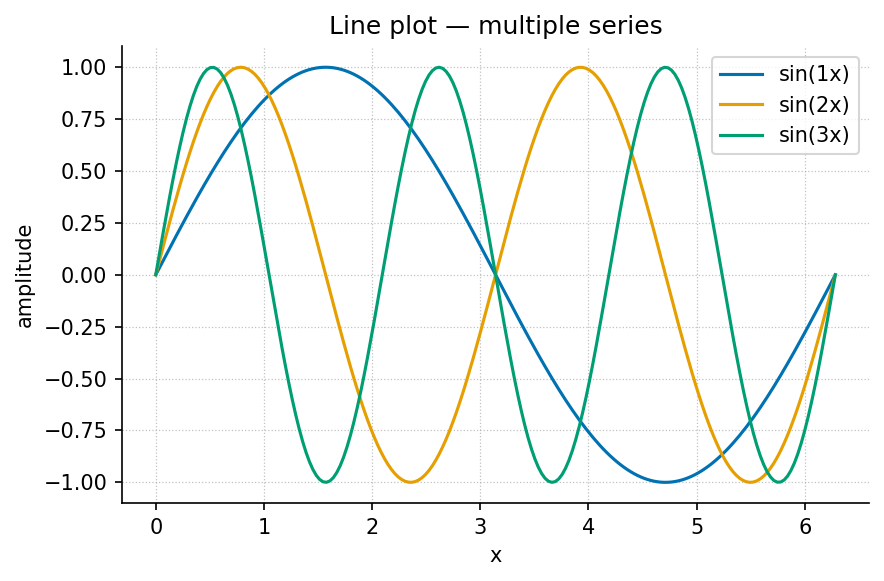
\includegraphics[width=0.8\linewidth,height=0.50\textheight,keepaspectratio,alt={A multi-series line plot of three sine waves, produced by visualization.gallery.line\_plot.}]{../figures/gallery/gallery_line.png}
\caption{A multi-series line plot of three sine waves, produced by
\protect\breaktt{visualization.gallery.line\_plot}.}\label{fig:gallery_line}
\end{figure}

Two figures side by side (Pandoc fenced div; falls back to stacked):

\begin{figure}
\centering
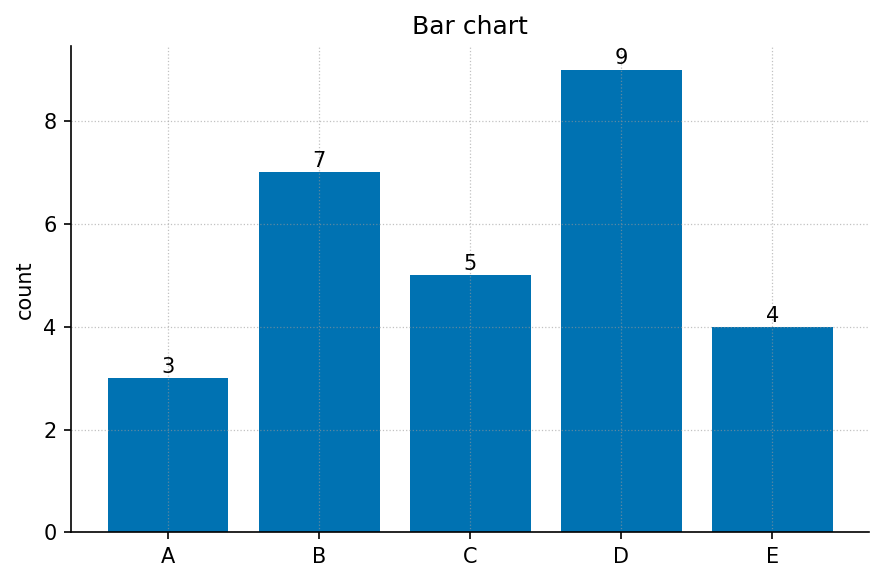
\includegraphics[width=0.48\linewidth,height=0.50\textheight,keepaspectratio,alt={Bar chart.}]{../figures/gallery/gallery_bar.png}
\caption{Bar chart.}\label{fig:gallery_bar}
\end{figure}

\begin{figure}
\centering
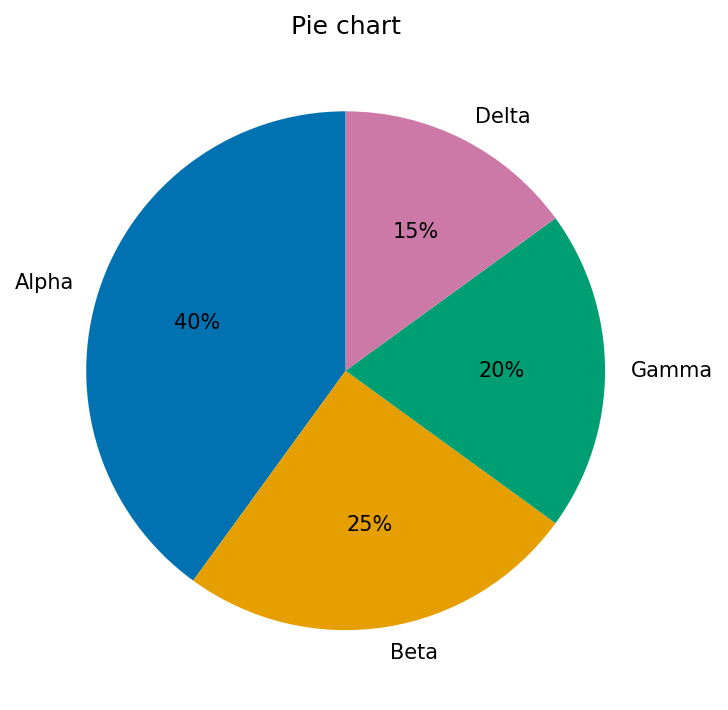
\includegraphics[width=0.48\linewidth,height=0.50\textheight,keepaspectratio,alt={Pie chart.}]{../figures/gallery/gallery_pie.png}
\caption{Pie chart.}\label{fig:gallery_pie}
\end{figure}

A multi-panel composite (fig.~\ref{fig:gallery_multipanel}):

\begin{figure}
\centering
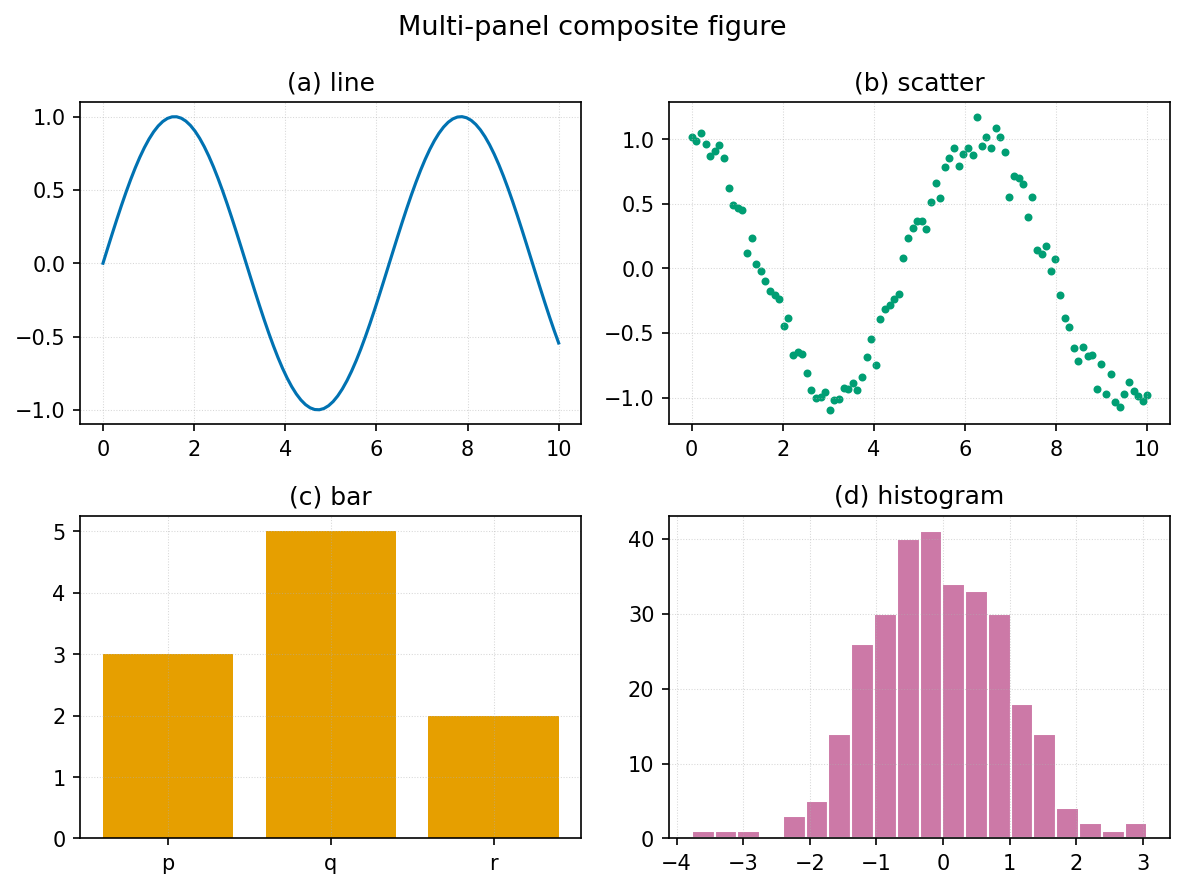
\includegraphics[width=0.85\linewidth,height=0.50\textheight,keepaspectratio,alt={A 2\texorpdfstring{\ensuremath{\times}}{x}2 composite: line, scatter, bar, and histogram panels.}]{../figures/gallery/gallery_multipanel.png}
\caption{A 2\texorpdfstring{\ensuremath{\times}}{x}2 composite: line, scatter, bar, and histogram
panels.}\label{fig:gallery_multipanel}
\end{figure}

The full plot-type gallery lives in \breaktt{../figures/gallery/} and
includes: line, scatter-with-fit, bar, grouped bar, horizontal bar,
histogram, box, violin, heatmap, contour, quiver field, step, stacked
area, error bars, log-log, pie, annotated, and multi-panel.

\begin{center}\rule{0.5\linewidth}{0.5pt}\end{center}

\subsection{7. Diagrams (Mermaid)}\label{diagrams-mermaid}

The pipeline renders fenced \texttt{mermaid} blocks to figures (and
falls back to the \texttt{.mmd} source if the Mermaid CLI is absent).
One worked example of each kind the builders in
\breaktt{src/mermaid/diagrams.py} support:

Flowchart:

\begin{figure}[htbp]
\centering
\begin{verbatim}
graph TD
  A[Inputs] --> B[Model]
  B --> C[Predictions]
  C -->|revise| A
\end{verbatim}
\caption{Mermaid diagram}
\end{figure}

Sequence:

\begin{figure}[htbp]
\centering
\begin{verbatim}
sequenceDiagram
  participant Author
  participant Engine
  Author ->> Engine: edit config.yaml
  Engine -->> Author: rendered PDF
\end{verbatim}
\caption{Mermaid diagram}
\end{figure}

State:

\begin{figure}[htbp]
\centering
\begin{verbatim}
stateDiagram-v2
  [*] --> Stub
  Stub --> Drafted: fill
  Drafted --> Reviewed: review
  Reviewed --> [*]: publish
\end{verbatim}
\caption{Mermaid diagram}
\end{figure}

Class:

\begin{figure}[htbp]
\centering
\begin{verbatim}
classDiagram
  class ChapterRef {
    +str part_id
    +str file
    +stem() str
  }
  ChapterRef --> TocEntry : numbered as
\end{verbatim}
\caption{Mermaid diagram}
\end{figure}

Entity-relationship:

\begin{figure}[htbp]
\centering
\begin{verbatim}
erDiagram
  PART ||--o{ CHAPTER : contains
  CHAPTER ||--|| LAB : has
\end{verbatim}
\caption{Mermaid diagram}
\end{figure}

Pie, Gantt, mindmap, timeline, quadrant, and user-journey diagrams are
also supported --- see \breaktt{src/mermaid/diagram\_specs.yaml} for a
worked spec of each.

\begin{center}\rule{0.5\linewidth}{0.5pt}\end{center}

\subsection{8. Code}\label{code}

Inline code: call
\breaktt{textbook.models.logistic\_growth(t,\ r=...,\ ...)}.

A fenced code block with a language (syntax-highlighted) and a caption
(lst.~\ref{lst:gallery_code}):

\begin{codelisting}

\caption{Calling the tested computational
backbone.}\label{lst:gallery_code}

\begin{Shaded}
\begin{Highlighting}[]
\ImportTok{from}\NormalTok{ textbook }\ImportTok{import}\NormalTok{ models}
\ImportTok{import}\NormalTok{ numpy }\ImportTok{as}\NormalTok{ np}

\NormalTok{t }\OperatorTok{=}\NormalTok{ np.linspace(}\DecValTok{0}\NormalTok{, }\DecValTok{10}\NormalTok{, }\DecValTok{100}\NormalTok{)}
\NormalTok{n }\OperatorTok{=}\NormalTok{ models.logistic\_growth(t, r}\OperatorTok{=}\FloatTok{0.8}\NormalTok{, carrying\_capacity}\OperatorTok{=}\FloatTok{100.0}\NormalTok{, initial}\OperatorTok{=}\FloatTok{5.0}\NormalTok{)}
\BuiltInTok{print}\NormalTok{(n[}\OperatorTok{{-}}\DecValTok{1}\NormalTok{])  }\CommentTok{\# {-}\textgreater{} approaches the carrying capacity}
\end{Highlighting}
\end{Shaded}

\end{codelisting}

A shell example:

\begin{Shaded}
\begin{Highlighting}[]
\ExtensionTok{uv}\NormalTok{ run python scripts/generate\_figures.py}
\ExtensionTok{uv}\NormalTok{ run }\AttributeTok{{-}{-}extra}\NormalTok{ dev python }\AttributeTok{{-}m}\NormalTok{ pytest tests/ }\AttributeTok{{-}{-}cov}\OperatorTok{=}\NormalTok{src}
\end{Highlighting}
\end{Shaded}

\begin{center}\rule{0.5\linewidth}{0.5pt}\end{center}

\subsection{9. Cross-references and
citations}\label{cross-references-and-citations}

Cross-references resolve by label: figure fig.~\ref{fig:gallery_line},
table tbl.~\ref{tbl:gallery_alignment}, equation
eq.~\ref{eq:gallery_logistic}, and section
sec.~\ref{sec:appendix_formalisms}. Never hand-number --- Pandoc fills
these in.

Citations resolve against \texttt{references.bib}: a single source
\citep{smith2020foundations}, multiple sources
\citep{doe2019methods, lee2021systems}, and an in-text form ---
\citet{garcia2022dynamics} showed the effect first. A locator narrows
the reference \citep[pp.~12--14]{patel2018models}.

\begin{center}\rule{0.5\linewidth}{0.5pt}\end{center}

\subsection{10. Media and data}\label{media-and-data}

Embedded raster image (any PNG/JPG works the same way as a figure):

\begin{figure}
\centering
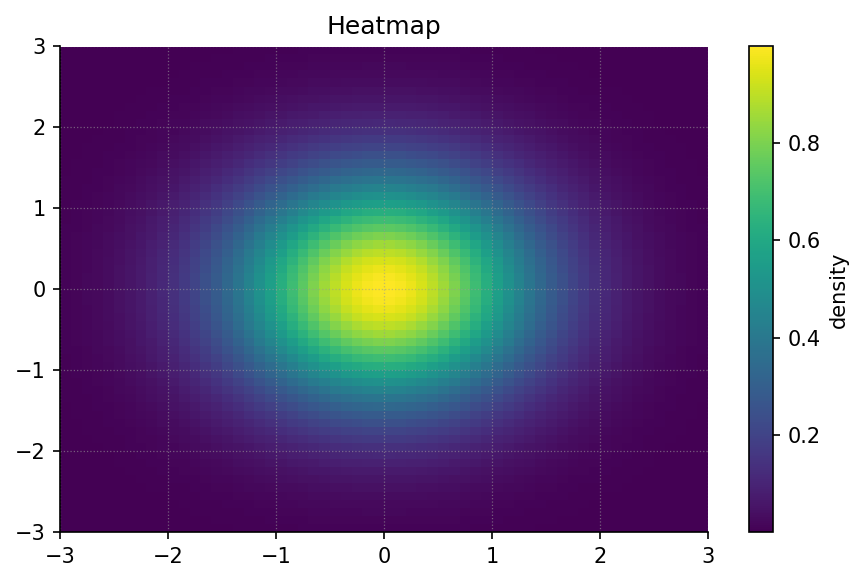
\includegraphics[width=0.6\linewidth,height=0.50\textheight,keepaspectratio,alt={A generated heatmap embedded as a raster image.}]{../figures/gallery/gallery_heatmap.png}
\caption{A generated heatmap embedded as a raster
image.}\label{fig:gallery_media}
\end{figure}

Audio and video embed in HTML targets (PDF shows the caption + link).
Syntax:

\begin{Shaded}
\begin{Highlighting}[]
\AlertTok{![Caption for an audio clip.](../assets/media/clip.mp3)}
\AlertTok{![Caption for a video.](../assets/media/demo.mp4)}\NormalTok{\{width=70\%\}}
\end{Highlighting}
\end{Shaded}

A downloadable data file lives at
\href{../assets/data/sample_dataset.csv}{\breaktt{assets/data/sample\_dataset.csv}};
its contents as a table:

\begin{longtable}[]{@{}lrrr@{}}
\caption{Sample dataset (mirrors
\protect\breaktt{assets/data/sample\_dataset.csv}).}\label{tbl:gallery_data}\tabularnewline
\toprule\noalign{}
condition & replicate & measurement & standard\_error \\
\midrule\noalign{}
\endfirsthead
\toprule\noalign{}
condition & replicate & measurement & standard\_error \\
\midrule\noalign{}
\endhead
\bottomrule\noalign{}
\endlastfoot
control & 1 & 2.10 & 0.20 \\
control & 2 & 2.30 & 0.18 \\
treatment\_low & 1 & 3.60 & 0.25 \\
treatment\_high & 1 & 4.80 & 0.35 \\
\end{longtable}

The error-bar figure fig.~\ref{fig:gallery_errorbar} visualises this
kind of data:

\begin{figure}
\centering
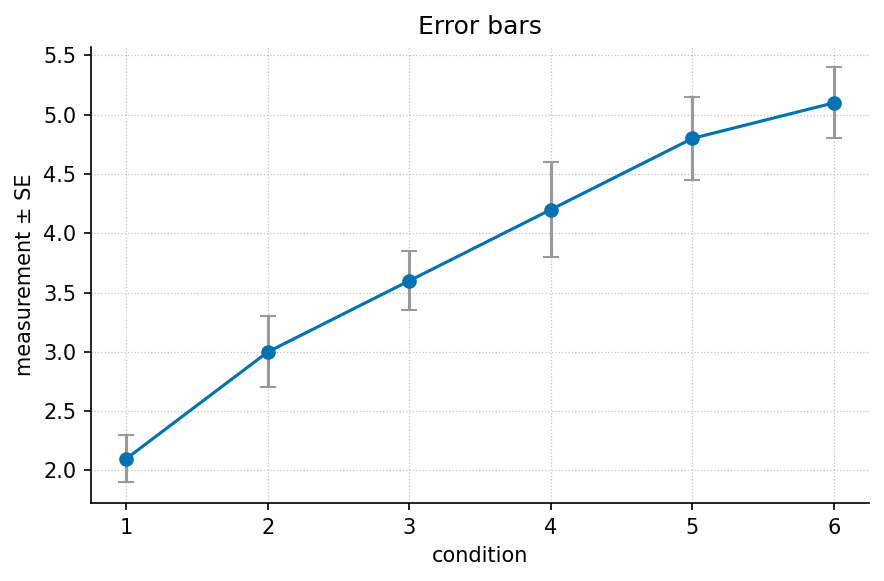
\includegraphics[width=0.7\linewidth,height=0.50\textheight,keepaspectratio,alt={Means with standard-error bars.}]{../figures/gallery/gallery_errorbar.png}
\caption{Means with standard-error bars.}\label{fig:gallery_errorbar}
\end{figure}

\begin{center}\rule{0.5\linewidth}{0.5pt}\end{center}

\subsection{11. Pedagogical blocks}\label{pedagogical-blocks}

These are the reusable teaching elements chapters draw on.

\begin{quote}
\textbf{Learning objective.} After this section a reader can identify
which Markdown primitive to use for a given purpose.
\end{quote}

\begin{quote}
\textbf{Worked example.} Given \(r = 0.8\), \(K = 100\), \(N_0 = 5\),
evaluate \(N(10)\) via eq.~\ref{eq:gallery_logistic} using
\breaktt{textbook.models.logistic\_growth}. The result approaches \(K\).
\end{quote}

\begin{quote}
\textbf{Try it.} Change \(r\) to \(1.5\) and predict, then check, how
the curve shifts.
\end{quote}

\begin{quote}
\textbf{Key terms.} \hyperref[gl:model]{\textbf{model}},
\hyperref[gl:parameter]{\textbf{parameter}},
\hyperref[gl:state]{\textbf{state}}.
\end{quote}

\begin{quote}
\textbf{Summary.} This appendix demonstrated text, lists, callouts,
tables, math and units, figures, diagrams, code, cross-references,
media, and pedagogy blocks --- the complete primitive set.
\end{quote}

\begin{center}\rule{0.5\linewidth}{0.5pt}\end{center}

\subsection{12. Miscellany}\label{miscellany}

A horizontal rule separates major shifts in topic (three or more
dashes):

\begin{center}\rule{0.5\linewidth}{0.5pt}\end{center}

Raw inline HTML is supported only inside
\texttt{\textless{}details\textgreater{}},
\texttt{\textless{}aside\textgreater{}}, or
\texttt{\textless{}callout\textgreater{}} per project style; everything
else uses Markdown. Unicode renders directly: \texorpdfstring{\ensuremath{\alpha}}{alpha}, \texorpdfstring{\ensuremath{\beta}}{beta}, \texorpdfstring{\ensuremath{\gamma}}{gamma}, \texorpdfstring{\ensuremath{\Delta}}{Delta}, ∑, \texorpdfstring{\ensuremath{\infty}}{inf}, \texorpdfstring{\ensuremath{\approx}}{~}, \texorpdfstring{\ensuremath{\to}}{->}.
For PDF math, prefer LaTeX (\texttt{\$\textbackslash{}alpha\$}) over raw
Unicode in equations.

\newpage

\section{Master Glossary}\label{master-glossary}

\subsubsection{Boundary}\label{gl:boundary}

The interface separating a system from its environment.

\subsubsection{Dynamics}\label{gl:dynamics}

How the state of a system changes over time.

\subsubsection{Emergence}\label{gl:emergence}

System-level behaviour not present in the parts taken alone.

\subsubsection{Equilibrium}\label{gl:equilibrium}

A state in which opposing influences balance and net change is zero.

\subsubsection{Feedback}\label{gl:feedback}

A loop in which a system's output influences its own input.

\subsubsection{Gradient}\label{gl:gradient}

A spatial or quantitative difference that drives flow or change.

\subsubsection{Model}\label{gl:model}

A simplified, often quantitative, representation of a system.

\subsubsection{Network}\label{gl:network}

A set of elements (nodes) connected by relationships (edges).

\subsubsection{Observable}\label{gl:observable}

A quantity that can be measured or recorded.

\subsubsection{Parameter}\label{gl:parameter}

A fixed quantity that configures a model's behaviour.

\subsubsection{Regulation}\label{gl:regulation}

The control of a system variable toward a target range.

\subsubsection{State}\label{gl:state}

The configuration of a system at a moment in time.

\subsubsection{System}\label{gl:system}

A set of interacting parts forming an integrated whole.

\subsubsection{Threshold}\label{gl:threshold}

A critical value at which a qualitative change occurs.

\subsubsection{Variable}\label{gl:variable}

A quantity that can take different values across states or observations.

\newpage

\section{Appendix E --- Index of Key Terms}\label{sec:appendix_index}

\begin{quote}
Reference appendix \texorpdfstring{\ensuremath{\cdot}}{.} Generated index --- do not hand-maintain.
\end{quote}

This index is intended to be \textbf{generated} at build time, not
edited by hand. A future indexing pass will scan the chapters for
glossary links
(\texttt{{[}**term**{]}(\#gl:\textless{}anchor\textgreater{})}) and
crossref labels (\texttt{\{\#sec:...\}}, \texttt{\{\#fig:...\}},
\texttt{\{\#tbl:...\}}, \texttt{\{\#eq:...\}}) and collate page/section
references from the rendered PDF. Until that pass runs, the entries
below are placeholders.

The authoritative term definitions live in
\href{../glossary.md}{Appendix D --- Glossary}; the closed list of
anchors is \breaktt{GLOSSARY\_ANCHORS} in
\href{../../src/textbook/constants.py}{\breaktt{src/textbook/constants.py}}.

\subsection{Placeholder Entries}\label{placeholder-entries}

\begin{itemize}
\tightlist
\item
  \textbf{dynamics} --- see sec.~\ref{sec:part_II_dynamics_and_change}
\item
  \textbf{equilibrium} --- see
  sec.~\ref{sec:part_II_regulation_and_control}
\item
  \textbf{feedback} --- see
  sec.~\ref{sec:part_II_regulation_and_control}
\item
  \textbf{model} --- see sec.~\ref{sec:part_0_quantitative_foundations}
\item
  \textbf{network} --- see sec.~\ref{sec:part_I_structure_and_form}
\item
  \textbf{system} --- see sec.~\ref{sec:part_II_systems_overview}
\end{itemize}

See also: \href{../glossary.md}{Appendix D --- Glossary}.



\clearpage

\bibliography{references}
\end{document}
